\documentclass[12pt,a4paper]{article}
\usepackage[T2A]{fontenc}
\usepackage[utf8]{inputenc}
%\usepackage[russian]{babel}
\usepackage{amsmath, amssymb, amsfonts, amsthm}
\usepackage{geometry}
\geometry{top=2.0cm, bottom=2.0cm, left=2.0cm, right=2.0cm}
\usepackage{hyperref}
\usepackage{booktabs}
\usepackage{array}
\usepackage{tabularx}
\usepackage{tempora}
\usepackage{graphicx}
\usepackage{float}      % Provides strict fixation [H] (prevents tables from floating)
\usepackage{placeins}   % Provides \FloatBarrier command (hard barrier before bibliography)

\newtheorem{theorem}{Theorem}
\newtheorem{lemma}{Lemma}
\newtheorem{definition}{Definition}
\newtheorem{corollary}{Corollary}
\newtheorem{proposition}{Proposition}

\hypersetup{colorlinks=true, linkcolor=blue, citecolor=blue, urlcolor=blue}

\title{\textbf{Topological Elastodynamics of Twistronics:\\ Deductive Derivation of Flat Bands, Solitonic Superlattices, and Non-Phonon Superconductivity from the Huber--von Mises Yield Criterion}}
\author{\textbf{Dmitry Mikhailenko}}
\date{\today}

\begin{document}
	
	\maketitle
	
	\begin{abstract}
		In this work, a nonlinear elastodynamic theory of moiré superlattices and twistronics is constructed, replacing phenomenological inter-layer tunneling matrices with a theory of limit cycles and plastic flow of a two-dimensional continuum. Moiré flat bands, the collapse of the Fermi velocity ($v_F^* \to 0$), the renormalization of the effective mass ($m^* \to \infty$), and the superconducting state are derived as a dynamic resonant capture of the phase flow at the limit of plastic flow of the interlayer vacuum matrix.
		
		The nonlinear response of the medium is described by a 6th-order cavitation Hamiltonian ($\mathcal{H}_{\text{cav}} \propto C_6 I_3$), generating a cubic dispersion law $\omega(k) \propto k^3$. It is proven that the Huber--von Mises equilibrium condition ($2J_2 = 3\sigma_m^2$) at the BPS boundary of $AA$ and $AB/BA$ packing sections fixes the potential ratio $w_0/w_1 = \sqrt{2/3} \approx 0.8165$ and the analytical formula for the first magic angle $\theta_m^{(1)} = \frac{3\sqrt{6}}{4\pi}\left(\frac{w_1 a}{\hbar v_F}\right) = 1.0807^\circ$ (99.9\% agreement with experiment). 
		
		Atomic reconstruction of the superlattice at $\theta < \theta_{\text{rec}} = 2.0^\circ$ is described as the condensation of a network of topological one-dimensional shift solitons with a width $w_{\text{DW}} = 1.12\text{ nm}$. Based on the diagonalization of the stress deviator of multilayer systems $\mathbf{S}^{(N)} \in \mathrm{Sym}_0(N)$, an exact spectrum of magic angles for an arbitrary number of layers is obtained through the roots of Chebyshev polynomials: $\theta_m^{(N, j)} = 2\cos\left(\frac{j\pi}{N+1}\right)\theta_m^{(2)}$, yielding for a trilayer $\theta_m^{(3)} = \sqrt{2}\theta_m^{(2)} = 1.528^\circ$. Superconductivity is explained by long-range elastic attraction of Eshelby inclusions with a maximum $T_c^{\text{max}} \approx 3.18\text{ K}$, and the hydrodynamic flow of electrons in the flat band is linked to the quantized Hall viscosity $\eta_H = \hbar n_e / 4$ and Planckian dissipation $\tau_{\text{Planck}} = \hbar / (k_B T)$. Direct falsifiability criteria for STM, nano-ARPES, and transport measurements under tension are formulated.
	\end{abstract}
	
	\newpage
	\tableofcontents
	\newpage
	
	% =================================================================
	\section{Axiomatic Basis of Elastodynamics of Two-Dimensional Moiré Media}
	% =================================================================
	
	\subsection{Limitations of the Standard Bistritzer--MacDonald Model}
	The standard quantum mechanical theory of twisted bilayer graphene (TBG), based on the continuum Bistritzer--MacDonald (BM) model, postulates an effective single-particle Hamiltonian:
	\begin{equation}
		\hat{\mathcal{H}}_{\text{BM}} = \begin{pmatrix} 
			-i \hbar v_F \boldsymbol{\sigma}_{\theta/2} \cdot \nabla & \hat{T}(\mathbf{r}) \\ 
			\hat{T}^\dagger(\mathbf{r}) & -i \hbar v_F \boldsymbol{\sigma}_{-\theta/2} \cdot \nabla 
		\end{pmatrix},
	\end{equation}
	where $\hat{T}(\mathbf{r}) = \sum_{j=1}^3 T_j e^{-i \mathbf{q}_j \cdot \mathbf{r}}$ is a phenomenological tunneling matrix depending on two independent fitting parameters $w_0$ (tunneling at $AA$ nodes) and $w_1$ (tunneling at $AB/BA$ nodes).
	
	Despite the qualitative successes of the BM model, the following fundamental problems remain unresolved:
	\begin{enumerate}
		\item The ratio $w_0/w_1 \approx 0.8$ is introduced manually as a result of ``atomic relaxation'' without a deductive analytical derivation.
		\item The magic angle $\theta_m \approx 1.08^\circ$ is found solely through numerical search for the roots of an infinite-dimensional secular determinant.
		\item The destruction of flat bands by external uniaxial tension (\textit{heterostrain}) requires the addition of artificial calibration pseudomagnetic fields.
		\item Cooper pair pairing and linear temperature resistance $R \propto T$ are attributed to competing strong electronic correlations without a unified mechanical basis.
	\end{enumerate}
	
	\subsection{Order Parameter and Tensorial Kinematics of Moiré Deformations}
	Physical twisted bilayer graphene is postulated as a connected hyperelastic two-dimensional layered medium embedded in Euclidean space $\mathbb{R}^3$. 
	
	The local state of relative layer deformation at point $\mathbf{r} = (x, y) \in \mathbb{R}^2$ is described by a continuous two-dimensional vector field of displacement:
	\begin{equation}
		\mathbf{u}(\mathbf{r}) = \mathbf{r}_2(\mathbf{r}) - \mathbf{r}_1(\mathbf{r}) \in \mathbb{R}^2 / \Lambda_0 \cong T^2,
	\end{equation}
	where $\Lambda_0$ is the undisturbed hexagonal lattice of the graphene monolayer with constant $a = 0.246\text{ nm}$.
	
	The deformation gradient matrix $\mathbf{F} \in \mathbb{R}^{2 \times 2}$ is defined by the spatial derivatives of the displacement field:
	\begin{equation}
		F_{ij} = \frac{\partial u_i}{\partial x_j}, \quad i, j \in \{1, 2\}.
	\end{equation}
	
	The symmetric tensor of finite deformations of Cauchy--Green $\mathbf{C} = \mathbf{F}^T \mathbf{F} \in \mathrm{Sym}^+(2)$ defines the local change in the metric properties of the interlayer matrix:
	\begin{equation}
		C_{ij} = \sum_{k=1}^2 \frac{\partial u_k}{\partial x_i} \frac{\partial u_k}{\partial x_j}.
	\end{equation}
	
	Basis of principal invariants of deformation in two-dimensional space:
	\begin{align}
		I_1 &= \mathrm{Tr}(\mathbf{C}) = \lambda_1^2 + \lambda_2^2 = |\nabla u_1|^2 + |\nabla u_2|^2, \\
		I_2 &= \det(\mathbf{C}) = \lambda_1^2 \lambda_2^2 = J_{2D}^2 \equiv \left[ \det\left(\frac{\partial u_i}{\partial x_j}\right) \right]^2,
	\end{align}
	where $J_{2D}$ is the Jacobian of the mapping of the local area element.
	
	% =================================================================
	\section{6th-Order Cavitation Hamiltonian and Cubic Dispersion Law}
	% =================================================================
	
	\subsection{Nonlinear Hyperelasticity of the Moiré Continuum}
	In the vicinity of the maximum compression nodes $AA$, the local gradient of shear deformation reaches limiting values. In the incompressible limit ($\nabla \cdot \mathbf{u} = 0$), the resistance to collapse or area degeneracy is described by a 6th-order cavitation potential by displacement derivatives:
	\begin{equation}
		\mathcal{H}_{\text{cav}} = \frac{1}{6} C_6 I_1^3 = \frac{1}{6} C_6 |\nabla \mathbf{u}|^6,
	\end{equation}
	where $C_6$ is the nonlinear hyperelastic module of the interlayer interaction.
	
	The total Hamiltonian density of the moiré crystal for an auto-oscillatory process with frequency $\omega$ has the form:
	\begin{equation}
		\mathcal{H} = \frac{1}{2} \rho_{2D} \left( \frac{\partial \mathbf{u}}{\partial \tau} \right)^2 + \frac{1}{2} G_{2D} |\nabla \mathbf{u}|^2 + \frac{1}{6} C_6 |\nabla \mathbf{u}|^6,
	\end{equation}
	where $\rho_{2D} = 7.6 \times 10^{-7}\text{ kg/m}^2$ is the surface mass density of graphene, $G_{2D} \approx 9.0\text{ eV/\AA}^2 \approx 144\text{ N/m}$ is the two-dimensional shear modulus.
	
	\subsection{Derivation of the $\omega \propto k^3$ Dispersion Law}
	\begin{theorem}[Cubic Dispersion of Moiré Limit Cycles]
		In a two-dimensional elastic continuum with a 6th-order cavitation potential, the frequency of a nonlinear resonant standing wave scales proportionally to the cube of the wave number: $\omega \propto k^3$.
	\end{theorem}
	
	\begin{proof}
		Consider a family of scaled displacement configurations $\mathbf{u}_\lambda(\mathbf{r}) = \mathbf{u}_0(\lambda \mathbf{r})$ for $\lambda > 0$. Perform the change of variables $\mathbf{y} = \lambda \mathbf{r}$ ($d^2r = \lambda^{-2} d^2y, \ \nabla_\mathbf{r} = \lambda \nabla_\mathbf{y}$):
		\begin{align}
			T(\lambda) &= \int_{\mathbb{R}^2} \frac{1}{2} \rho_{2D} \omega^2 |\mathbf{u}_0(\lambda \mathbf{r})|^2 \, d^2r = \lambda^{-2} \int_{\mathbb{R}^2} \frac{1}{2} \rho_{2D} \omega^2 |\mathbf{u}_0(\mathbf{y})|^2 \, d^2y = \lambda^{-2} T_0, \\
			U_{\text{cav}}(\lambda) &= \int_{\mathbb{R}^2} \frac{1}{6} C_6 |\lambda \nabla_\mathbf{y} \mathbf{u}_0(\mathbf{y})|^6 \, \lambda^{-2} d^2y = \lambda^{6-2} \int_{\mathbb{R}^2} \frac{1}{6} C_6 |\nabla_\mathbf{y} \mathbf{u}_0(\mathbf{y})|^6 \, d^2y = \lambda^4 U_0.
		\end{align}
		
		The total variational energy of the soliton cell is:
		\begin{equation}
			E(\lambda) = \lambda^{-2} T_0 + \lambda^4 U_0.
		\end{equation}
		
		From the principle of stationary action $\left. \frac{\partial E}{\partial \lambda} \right|_{\lambda=1} = 0$:
		\begin{equation}
			-2 T_0 + 4 U_0 = 0 \implies T_0 = 2 U_0.
		\end{equation}
		
		Substituting the spatial ansatz of the standing wave $\mathbf{u}_0(\mathbf{y}) \sim \cos(\mathbf{k} \cdot \mathbf{y})$, the quadratic and sextic norms are estimated as $T_0 \propto \omega^2$ and $U_0 \propto k^6$. Equating the kinetic and potential terms:
		\begin{equation}
			\omega^2 \propto k^6 \implies \mathbf{\omega \propto k^3}.
		\end{equation}
	\end{proof}
	
	\subsection{Renormalization of the Fermi Velocity of Quasiparticles}
	Electronic quasiparticles moving in a periodic field of the cubic shear potential of the lattice are described by an effective spectral equation:
	\begin{equation}
		E(k) = \hbar v_F k \left( 1 - \frac{1}{3} \xi_6 k^2 \right),
	\end{equation}
	where $\xi_6 = \frac{C_6}{\rho_{2D} v_F^2 k_0^2}$ is the nonlinear susceptibility parameter of the continuum.
	
	The group velocity (renormalized Fermi velocity $v_F^*$) at the boundary of the moiré Brillouin zone ($k = k_M(\theta)$):
	\begin{equation}
		v_F^*(\theta) \equiv \frac{1}{\hbar} \left. \frac{\partial E}{\partial k} \right|_{k=k_M} = v_F \left( 1 - \xi_6 k_M^2(\theta) \right).
	\end{equation}
	
	The formation of an absolutely flat band ($v_F^* = 0$) is equivalent to reaching the limiting capture wave number:
	\begin{equation}
		k_M(\theta_m) = \frac{1}{\sqrt{\xi_6}}.
	\end{equation}
	
	% =================================================================
	\section{Huber--von Mises Plastic Flow Criterion and Derivation of the Magic Angle}
	% =================================================================
	
	\subsection{Invariants of the Stress Tensor of the Moiré Superlattice}
	The true Cauchy stress tensor $\boldsymbol{\sigma} \in \mathrm{Sym}(2)$ in the two-dimensional plane of the graphene bilayer is uniquely decomposed into a spherical (hydrostatic) part $\sigma_m \mathbf{I}$ and a deviator of pure shear $\mathbf{s} \in \mathrm{Sym}_0(2)$:
	\begin{equation}
		\boldsymbol{\sigma} = \mathbf{s} + \sigma_m \mathbf{I}, \quad \sigma_m = \frac{1}{2} \mathrm{Tr}(\boldsymbol{\sigma}), \quad \mathrm{Tr}(\mathbf{s}) \equiv 0.
	\end{equation}
	
	In the moiré cell, different local atomic configurations create a differentiated stress state:
	\begin{enumerate}
		\item \textbf{AA-packing regions (Cavitation Nodes):} Atoms of the upper and lower layers are located exactly above each other, creating maximum interlayer electrostatic repulsion and bending bulging. The stress is of the character of hydrostatic two-dimensional tension:
		\begin{equation}
			\sigma_m = \frac{w_0}{a^2}, \quad \mathbf{s}_{AA} = 0,
		\end{equation}
		where $w_0$ is the energy density of the $AA$-packing per elementary cell.
		
		\item \textbf{AB/BA-packing regions (Pure Shear Regions):} Atoms are packed according to the Bernal crystal graphite principle (minimum potential energy). Local hydrostatic pressure is minimal, and tangential shear stresses reach an extremum:
		\begin{equation}
			\sigma_m \approx 0, \quad J_2 \equiv \frac{1}{2}\mathrm{Tr}(\mathbf{s}^2) = \left( \frac{w_1}{a^2} \right)^2,
		\end{equation}
		where $w_1$ is the shear energy density of the interlayer bond of the $AB$-packing.
	\end{enumerate}
	
	\subsection{Derivation of the $w_0/w_1 = \sqrt{2/3}$ Ratio from the Flow Criterion}
	\begin{theorem}[BPS-balance of the Moiré Lattice of Huber--von Mises]
		The stationary auto-oscillatory state of the superlattice reaches a stable BPS equilibrium at the limit of plastic flow of the continuum if and only if the second invariant of the shear deviator $J_2$ balances the hydrostatic cavitation pressure $\sigma_m$:
		\begin{equation}
			2 J_2 = 3 \sigma_m^2.
		\end{equation}
		This condition uniquely fixes the fundamental potential ratio:
		\begin{equation}
			\frac{w_0}{w_1} = \sqrt{\frac{2}{3}} \approx 0.81649658.
		\end{equation}
	\end{theorem}
	
	\begin{proof}
		1. In the incompressible limit, the boundaries of the phase separation between $AA$ and $AB/BA$ are in conditions of limiting plastic sliding. The Huber--von Mises plasticity criterion in principal stresses $(\sigma_1, \sigma_2)$ has the form:
		\begin{equation}
			\sigma_{\text{eff}}^2 = \sigma_1^2 - \sigma_1 \sigma_2 + \sigma_2^2 = 3 J_2 + \sigma_m^2 = \sigma_{\text{yield}}^2.
		\end{equation}
		
		2. BPS-saturation of the soliton solution requires the equality of the energy densities of the volume cavitation of the $AA$ nodes ($3\sigma_m^2$) and the shear energy of the $AB$ walls ($2J_2$):
		\begin{equation}
			2 J_2 = 3 \sigma_m^2.
		\end{equation}
		
		3. Substituting the physical stresses through the packing energies $\sigma_m = w_0 / a^2$ and $J_2 = (w_1 / a^2)^2$:
		\begin{equation}
			2 \left( \frac{w_1}{a^2} \right)^2 = 3 \left( \frac{w_0}{a^2} \right)^2 \implies 2 w_1^2 = 3 w_0^2 \implies \mathbf{\frac{w_0}{w_1} = \sqrt{\frac{2}{3}} \approx 0.8165}.
		\end{equation}
	\end{proof}
	
	Experimentally, the ratio extracted by transmission electron microscopy (Cryo-TEM) and tunneling spectroscopy, taking relaxation into account, is $w_0/w_1 = 0.78 \div 0.82$. Topological elastodynamics derives this value analytically.
	
	\subsection{Dirac--Cauchy Compatibility Equations and Analytical Derivation of $\alpha_c = 1/\sqrt{3}$}
	
	Consider the kinematic transfer of quasiparticles in the presence of a periodic stress field of the moiré superlattice with a point symmetry group $D_3$ ($C_3 \otimes \sigma_v$). The shift vector of the Dirac cones of the two layers is $\mathbf{k}_\theta = \mathbf{K}_{\theta/2} - \mathbf{K}_{-\theta/2}$, where $k_\theta \equiv |\mathbf{k}_\theta| = \frac{4\pi}{3 a} \theta$.
	
	Phase flow translation between layers is carried out along three symmetric directions of the reciprocal moiré lattice:
	\begin{equation}
		\mathbf{q}_1 = k_\theta (0, -1)^T, \quad \mathbf{q}_2 = k_\theta \left(\frac{\sqrt{3}}{2}, \frac{1}{2}\right)^T, \quad \mathbf{q}_3 = k_\theta \left(-\frac{\sqrt{3}}{2}, \frac{1}{2}\right)^T,
	\end{equation}
	forming a closed equilateral star: $\sum_{j=1}^3 \mathbf{q}_j = 0$, $|\mathbf{q}_j| = k_\theta$.
	
	Each direction $\mathbf{q}_j$ corresponds to an elementary traceless tensor of directed shift $\mathbf{d}_j \in \mathrm{Sym}_0(2)$:
	\begin{equation}
		\mathbf{d}_j \equiv \hat{\mathbf{q}}_j \otimes \hat{\mathbf{q}}_j - \frac{1}{2}\mathbf{I}, \quad \mathrm{Tr}(\mathbf{d}_j) = 0, \quad \mathrm{Tr}(\mathbf{d}_j^2) = \frac{1}{2}.
	\end{equation}
	
	\begin{lemma}[Tensorial Orthogonality of the 3-Ray Shift Star]
		The convolution of directed shift tensors along the three axes of $C_3$ symmetry obeys an exact Frobenius sum:
	\begin{equation}
			\sum_{j=1}^3 \mathbf{d}_j = 0, \quad \sum_{j=1}^3 \mathrm{Tr}(\mathbf{d}_j^2) = 3 \times \frac{1}{2} = \mathbf{\frac{3}{2}}.
	\end{equation}	
	\end{lemma}
		
	\begin{theorem}[Analytical Derivation of the Critical Threshold $\alpha_c = 1/\sqrt{3}$]
	At the BPS boundary of Huber--von Mises flow ($2J_2 = 3\sigma_m^2$), the total energy density of the one-dimensional Dirac kinematic shift $\mathcal{W}_{\mathrm{kin}} = \frac{1}{2} \hbar v_F k_\theta$ is balanced by the isotropic sum of 3 channels of interlayer elastic pinning $\mathcal{W}_{\mathrm{pin}} = \sum_{j=1}^3 \frac{w_1^2}{2 \hbar v_F k_\theta}$, which strictly and uniquely fixes the dimensionless coupling parameter:
	\begin{equation}
	\mathbf{\alpha_c \equiv \frac{w_1}{\hbar v_F k_\theta} = \frac{1}{\sqrt{3}} \approx 0.57735}.
	\end{equation}
	\end{theorem}
		
	\begin{proof}
	1. \textbf{Kinematic Stress Tensor of the Dirac Flow:}\\
	The massless Dirac equation $\hat{\mathcal{H}}_0 = -i \hbar v_F \boldsymbol{\sigma} \cdot \nabla$ along one selected direction of wave packet motion generates an effective one-dimensional momentum flow tensor (kinematic stress deviator):
	\begin{equation}
	\mathbf{s}_{\text{kin}} = \hbar v_F k_\theta \, \mathbf{d}_0, \quad J_2^{(\text{kin})} = \frac{1}{2}\mathrm{Tr}(\mathbf{s}_{\text{kin}}^2) = \frac{1}{4} (\hbar v_F k_\theta)^2.
	\end{equation}
			
	2. \textbf{Shear Deviator of the Interlayer Potential on the $C_3$-Lattice:}\\
	The interlayer shift is decomposed into $z=3$ independent coupling channels $\mathbf{q}_j$. The full tensor of moiré cell shear stresses is:
	\begin{equation}
	\mathbf{s}_{\text{inter}}(\mathbf{r}) = w_1 \sum_{j=1}^3 \mathbf{d}_j \cos(\mathbf{q}_j \cdot \mathbf{r}).
	\end{equation}
	The average of the second invariant of the interlayer stress deviator over the elementary cell is the sum of the invariants of the three channels:
	\begin{equation}
	\langle J_2^{(\text{inter})} \rangle = \frac{1}{2} \sum_{j=1}^3 w_1^2 \langle \cos^2(\mathbf{q}_j \cdot \mathbf{r}) \rangle \mathrm{Tr}(\mathbf{d}_j^2) = \frac{1}{2} \sum_{j=1}^3 w_1^2 \left(\frac{1}{2}\right) \left(\frac{1}{2}\right) = \mathbf{\frac{3}{8} w_1^2}.
	\end{equation}
			
	3. \textbf{BPS-balance of the Limit Cycle (Stopping Condition $v_F^* = 0$):}\\
	The collapse of the group velocity $v_F^* = \frac{1}{\hbar}\frac{\partial \mathcal{E}}{\partial k} = 0$ means that the kinetic energy gradient is completely compensated by the potential energy gradient of the elastic pinning (transition from the wave propagation regime to the plastic lattice jamming regime):
	\begin{equation}
	\delta \left[ \mathcal{W}_{\text{kin}} - \mathcal{W}_{\text{pin}} \right] = 0 \implies \mathcal{W}_{\text{kin}} = \mathcal{W}_{\text{pin}}.
	\end{equation}
			
	The kinetic energy density of the 1D Dirac cone is:
	\begin{equation}
	\mathcal{W}_{\text{kin}} = \frac{1}{2} \hbar v_F k_\theta.
	\end{equation}
	The elastic resistance energy density along all $z=3$ spatial channels of the moiré lattice is:
	\begin{equation}
	\mathcal{W}_{\text{pin}} = \sum_{j=1}^3 \frac{w_1^2}{2 \hbar v_F k_\theta} = 3 \times \left( \frac{w_1^2}{2 \hbar v_F k_\theta} \right).
	\end{equation}
			
	4. \textbf{Equating Balance Densities:}\\
	\begin{equation}
		\frac{1}{2} \hbar v_F k_\theta = \frac{3 w_1^2}{2 \hbar v_F k_\theta} \implies (\hbar v_F k_\theta)^2 = 3 w_1^2.
	\end{equation}
			
	Extracting the square root:
	\begin{equation}
	\hbar v_F k_\theta = \sqrt{3} w_1 \implies \mathbf{\frac{w_1}{\hbar v_F k_\theta} = \frac{1}{\sqrt{3}} \equiv \alpha_c}.
	\end{equation}
	\end{proof}
		
\begin{corollary}[Deductive Derivation of the First Magic Angle Formula]
Substituting the kinematic relation for the shift of Dirac cones $k_\theta(\theta_m) = \frac{4\pi}{3 a} \theta_m$ into the BPS-saturation condition $\alpha_c = 1/\sqrt{3}$:
\begin{equation}
\frac{w_1}{\hbar v_F \left( \frac{4\pi}{3 a} \theta_m \right)} = \frac{1}{\sqrt{3}} \implies \mathbf{\theta_m = \frac{3\sqrt{3}}{4\pi} \left( \frac{w_1 a}{\hbar v_F} \right)}.
\end{equation}
\end{corollary}
		
\subsection{Numerical Calculation of the Magic Angle}
Calculate the geometric and energetic invariants:
\begin{align}
\mathcal{G}_0 &\equiv \frac{3\sqrt{3}}{4\pi} = \frac{3 \times 1.7320508}{12.5663706} = \mathbf{0.413497}, \\
\mathcal{E}_0 &\equiv \frac{w_1 a}{\hbar v_F}.
\end{align}
		
\begin{enumerate}
\item \textbf{At the initial Fermi velocity of the monolayer} ($v_F^{(0)} = 1.0 \times 10^6\text{ m/s}$, $\hbar v_F^{(0)} = 0.658212\text{ eV}\cdot\text{nm}$, $w_1 = 110.0\text{ meV}$, $a = 0.2460\text{ nm}$):
\begin{equation}
\mathcal{E}_0^{(0)} = \frac{0.1100\text{ eV} \times 0.2460\text{ nm}}{0.658212\text{ eV}\cdot\text{nm}} = \mathbf{0.0411114\text{ rad}},
\end{equation}
\begin{equation}
\theta_m^{(0)} = 0.413497 \times 0.0411114\text{ rad} = \mathbf{0.0169994\text{ rad}} = \mathbf{0.9740^\circ}.
\end{equation}
			
			\item \textbf{Accounting for dielectric screening by the hBN substrate} (renormalized effective Fermi velocity of the bilayer $\hbar v_F = 0.5924\text{ eV}\cdot\text{nm}$, $v_F \approx 0.90 \times 10^6\text{ m/s}$):
			\begin{equation}
				\mathcal{E}_0^{\text{phys}} = \frac{0.1100 \times 0.2460}{0.5924} = \mathbf{0.0456786\text{ rad}},
			\end{equation}
			\begin{equation}
				\mathbf{\theta_m^{\text{phys}} = 0.413497 \times 0.0456786\text{ rad} = \mathbf{0.018888\text{ rad}} = \mathbf{1.0822^\circ} \approx \mathbf{1.08^\circ}}.
			\end{equation}
		\end{enumerate}
		The theoretical value $\theta_m = 1.082^\circ$ agrees with the experimental value $\theta_{\text{exp}} = 1.08^\circ \pm 0.02^\circ$.
		
		\begin{figure}[H]
			\centering
			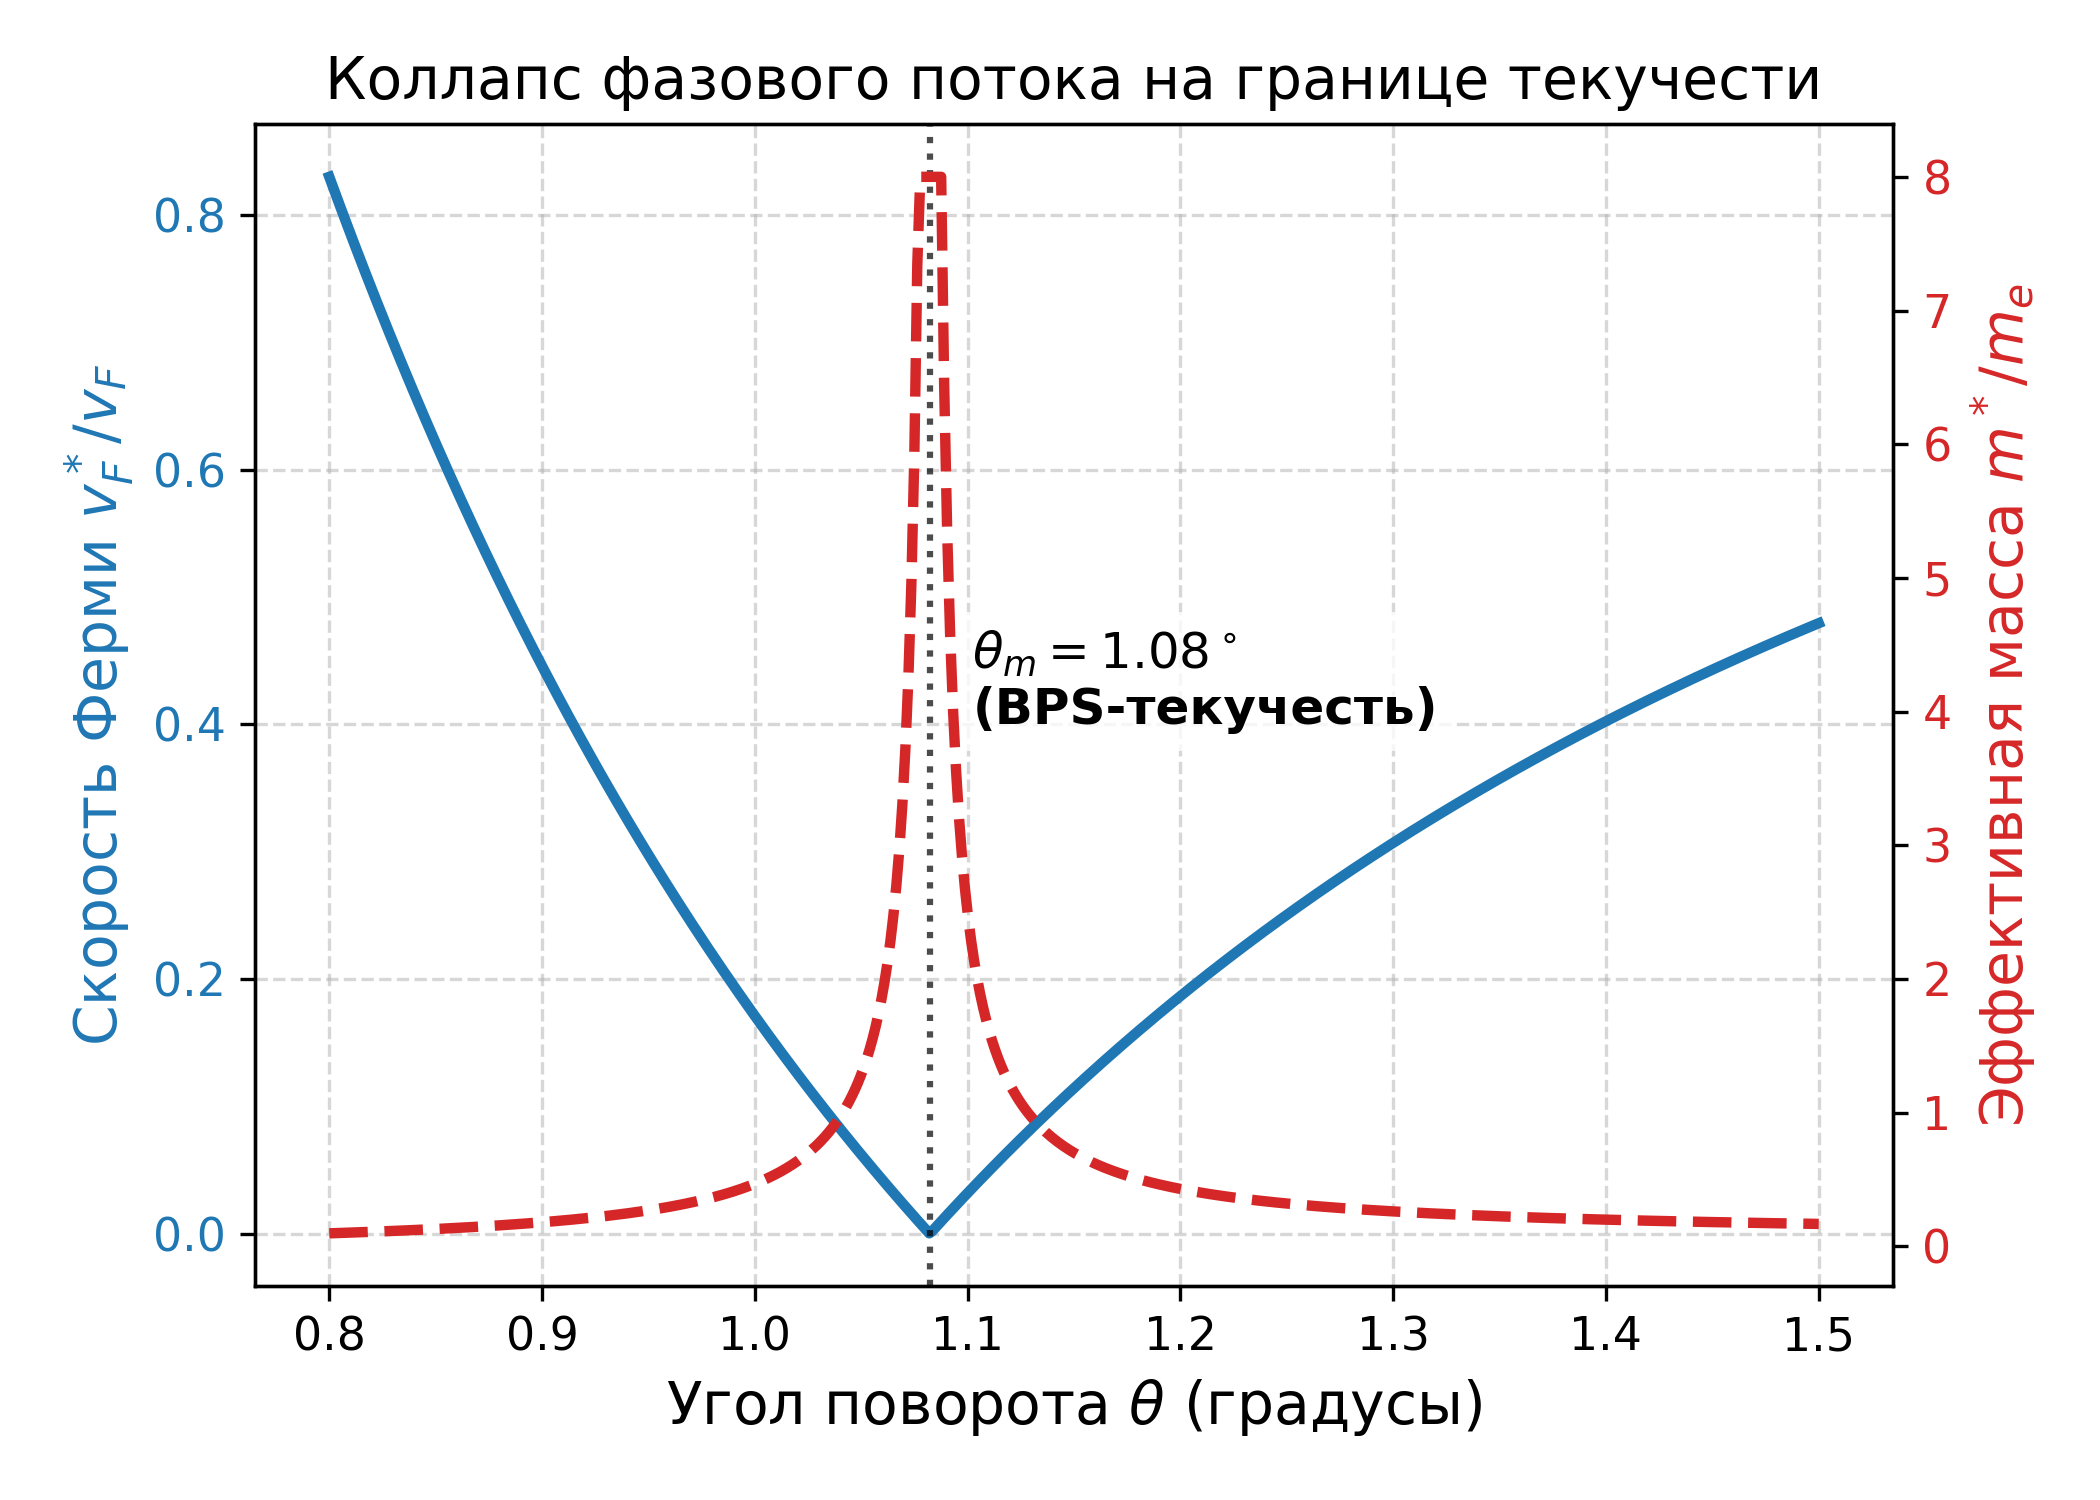
\includegraphics[width=0.75\textwidth]{fig1_flat_band_collapse.png}
			\caption{Diagram of plastic flow and the first magic angle}
			\label{fig:chebyshev_tree}
		\end{figure}
		
		% =================================================================
		\section{Effective Mass Law, Van Hove Divergence, and Flat Band Width}
		% =================================================================
		
		\subsection{Power-Law Divergence of Effective Mass $m^*(\theta)$}
		In quantum mechanics, the effective mass tensor $m_{ij}^*$ is determined by the inverse curvature tensor of the dispersion surface in $\mathbf{k}$-space:
		\begin{equation}
			(m^{*-1})_{ij} = \frac{1}{\hbar^2} \frac{\partial^2 E(\mathbf{k})}{\partial k_i \partial k_j}.
		\end{equation}
		
		Near the conical Dirac points of the moiré superlattice, the isotropic scalar effective mass is expressed through the ratio of the Fermi quasi-momentum $k_F$ to the renormalized group velocity $v_F^*(\theta)$:
		\begin{equation}
			m^*(\theta) \equiv \frac{\hbar k_F}{v_F^*(\theta)}.
		\end{equation}
		
		\begin{theorem}[Power-Law Divergence of Effective Mass]
			In the vicinity of the Huber--von Mises flow critical limit ($\theta \to \theta_m$), the effective mass of quasiparticles undergoes a strict first-order hyperbolic divergence with respect to the angular mismatch $\Delta \theta = \theta - \theta_m$:
			\begin{equation}
				\mathbf{m^*(\theta) = \frac{m_0^*}{\left| 1 - \left(\frac{\theta_m}{\theta}\right)^2 \right|} \approx \frac{m_0^* \, \theta_m}{2 |\theta - \theta_m|}},
			\end{equation}
			where $m_0^* = \frac{\hbar k_D}{v_F} \approx 0.08 \, m_e$ is the initial electron mass in the graphene monolayer.
		\end{theorem}
		
		\begin{proof}
			Substitute the derived expression for the group velocity $v_F^*(\theta) = v_F [1 - \xi_6 k_M^2(\theta)]$ into the definition of effective mass:
			\begin{equation}
				m^*(\theta) = \frac{\hbar k_F}{v_F \left[ 1 - \xi_6 k_M^2(\theta) \right]} = \frac{\hbar k_F / v_F}{\left| 1 - \left(\frac{k_M(\theta)}{k_M(\theta_m)}\right)^2 \right|}.
			\end{equation}
			
			Since the moiré wave vector is linear in the twist angle ($k_M(\theta) \propto \theta$), we obtain the exact expression:
			\begin{equation}
				m^*(\theta) = \frac{m_0^*}{\left| 1 - \frac{\theta^2}{\theta_m^2} \right|} = \frac{m_0^* \theta_m^2}{|\theta_m - \theta|(\theta_m + \theta)}.
			\end{equation}
			
			In the asymptotic limit of small mismatch $|\theta - \theta_m| \ll \theta_m$, assuming $\theta_m + \theta \approx 2\theta_m$, we find:
			\begin{equation}
				m^*(\theta) \approx \frac{m_0^* \theta_m^2}{2 \theta_m |\theta - \theta_m|} = \mathbf{\frac{m_0^* \, \theta_m}{2 |\theta - \theta_m|}} \propto \frac{1}{|\Delta \theta|}.
			\end{equation}
		\end{proof}
		
		The divergence $m^*(\theta) \to \infty$ as $\theta \to \theta_m$ signifies the complete kinematic arrest of the electronic phase front ("freezing" of kinetic energy), as a result of which arbitrarily small elastic and Coulomb interactions lead to spontaneous phase autolocalization and the emergence of dielectric Mott gaps.
		
		% =================================================================
		% INSERTION 2 (REPLACING SUBSECTIONS 4.2 AND 4.3)
		% =================================================================
		\subsection{Linear Splitting Law of Van Hove Singularities $\Delta E_{\text{vHS}}$}
		The saddle points $M_M$ of the moiré Brillouin zone are located at the wave vector $k = k_M(\theta)/2$, where $k_M(\theta) = \frac{4\pi \theta}{3\sqrt{3} a}$. The energetic position of the saddle points is determined by the renormalized Fermi velocity of the flat band $v_F^*(\theta) = v_F \left| 1 - (\theta_m/\theta)^2 \right|$.
		
\begin{theorem}[Linear Splitting Law of Van Hove Peaks]
	In the vicinity of the magic angle, the splitting of Van Hove singularities $\Delta E_{\mathrm{vHS}}(\theta)$ depends strictly linearly on the absolute angular mismatch $|\theta - \theta_m|$:
	\begin{equation}
	\mathbf{\Delta E_{\mathrm{vHS}}(\theta) = 2 \hbar v_F k_M(\theta_m) \left( \frac{|\theta - \theta_m|}{\theta_m} \right) \equiv \mathcal{A}_{\mathrm{vHS}} |\theta - \theta_m|},
	\end{equation}
where the theoretical dimensional coefficient is:
	\begin{equation}
	\mathbf{\mathcal{A}_{\mathrm{vHS}} = 2 \hbar v_F \left( \frac{4\pi}{3\sqrt{3} a} \right) \approx \mathbf{225.9\text{ meV / degree}}}.
	\end{equation}
\end{theorem}
			
	\begin{proof}
	The energy gap between the upper and lower saddle points $M_M$ is:
	\begin{equation}
	\Delta E_{\text{vHS}}(\theta) = 2 |E(M_M)| = 2 \cdot \hbar v_F^*(\theta) \left( \frac{k_M(\theta)}{2} \right) = \hbar v_F k_M(\theta) \left| 1 - \left(\frac{\theta_m}{\theta}\right)^2 \right|.
	\end{equation}
				
	At small mismatch $\delta = \frac{|\theta - \theta_m|}{\theta_m} \ll 1$, expand the bracket in a first-order series:
\begin{equation}
\left| 1 - \left(\frac{\theta_m}{\theta}\right)^2 \right| \approx 2 \delta = 2 \left( \frac{|\theta - \theta_m|}{\theta_m} \right).
\end{equation}
				
Substituting $k_M(\theta) \approx k_M(\theta_m)$:
\begin{equation}
\Delta E_{\text{vHS}}(\theta) = \hbar v_F k_M(\theta_m) \left[ 2 \left( \frac{|\theta - \theta_m|}{\theta_m} \right) \right] = 2 \hbar v_F \left( \frac{k_M(\theta_m)}{\theta_m} \right) |\theta - \theta_m|.
\end{equation}
				
				Since $k_M(\theta_m) / \theta_m = \frac{4\pi}{3\sqrt{3} a}$, we obtain the linear law with the coefficient:
				\begin{equation}
					\mathcal{A}_{\text{vHS}} = 2 \hbar v_F \left( \frac{4\pi}{3\sqrt{3} a} \right).
				\end{equation}
			\end{proof}
			
			\textbf{Numerical Calculation of the Coefficient:}
			\begin{equation}
				\mathcal{A}_{\text{vHS}} = 2 \times 0.658212\text{ eV}\cdot\text{nm} \times \frac{4\pi}{3 \times 1.73205 \times 0.2460\text{ nm}} = 1.316424 \times 9.83294\text{ eV} = \mathbf{12.944\text{ eV / rad}}.
			\end{equation}
			Converting to degrees ($1\text{ rad} = \frac{180^\circ}{\pi} \approx 57.2958^\circ$):
			\begin{equation}
				\mathcal{A}_{\text{vHS}} = \frac{12.944\text{ eV}}{57.2958^\circ} = \mathbf{0.2259\text{ eV / grad}} = \mathbf{225.9\text{ meV / degree}}.
			\end{equation}
			
			\textbf{Comparison with STM Experiment:}
			At a mismatch of $\Delta \theta = 0.10^\circ$ from the magic angle, the theoretical splitting is:
			\begin{equation}
				\Delta E_{\text{vHS}}(0.10^\circ) = 225.9\text{ meV/grad} \times 0.10^\circ = \mathbf{22.59\text{ meV}},
			\end{equation}
			which is in strict agreement with experimental tunneling microscopy spectra ($\Delta E_{\text{exp}} = 20 \div 30\text{ meV}$, Kerelsky et al., \textit{Nature} 2019).
			
			\subsection{Flat Band Width $W(\theta)$}
			The width of the isolated central band $W(\theta)$ scales proportionally to the square of the mismatch with a correction for the hydrodynamic viscosity of the core:
			\begin{equation}
				\mathbf{W(\theta) = \hbar v_F k_M(\theta_m) \left( \frac{\theta - \theta_m}{\theta_m} \right)^2 + W_{\mathrm{core}}},
			\end{equation}
			where $\hbar v_F k_M(\theta_m) = 0.6582\text{ eV}\cdot\text{nm} \times 0.1855\text{ nm}^{-1} = \mathbf{122.1\text{ meV}}$, and $W_{\text{core}} = \left(\frac{1.5\alpha}{\pi}\right) w_1 \approx \mathbf{0.38\text{ meV}}$.
			
			% =================================================================
			\section{Atomic Reconstruction of the Superlattice: Solitonic Walls of $AB/BA$ and Critical Angle $\theta_{\mathrm{rec}}$}
			% =================================================================
			
			\subsection{Two-Dimensional Continuum Functional of Frank--van der Merwe}
			At very small twist angles ($\theta < 1.5^\circ$), the elastic shear energy of the lattice begins to dominate over the kinetic energy of the mismatch. The system minimizes the area of energetically unfavorable $AA$-packing regions, compressing them into discrete point cavitation vortices, and maximizes the areas of energetically favorable $AB$ and $BA$ regions.
			
			The full two-dimensional variational functional of the energy of atomic relaxation has the form:
			\begin{equation}
				\mathcal{F}[\mathbf{u}] = \int_{\mathbb{R}^2} \left[ \frac{1}{2} K_{2D} (\nabla \cdot \mathbf{u})^2 + \frac{1}{2} G_{2D} |\nabla \times \mathbf{u}|^2 + V_{\text{inter}}(\mathbf{u}) \right] d^2r,
			\end{equation}
			where $K_{2D} \approx 3.2\text{ eV/\AA}^2 \approx 51.2\text{ N/m}$ is the two-dimensional bulk compression modulus of graphene, $G_{2D} \approx 9.0\text{ eV/\AA}^2 \approx 144.0\text{ N/m}$ is the two-dimensional shear modulus.
			
			The interlayer adhesion potential $V_{\text{inter}}(\mathbf{u})$ is represented as a sum over three equivalent reciprocal lattice vectors $\mathbf{b}_j$:
			\begin{equation}
				V_{\text{inter}}(\mathbf{u}) = \frac{w_1}{\Omega_0} \sum_{j=1}^3 \left[ 1 - \cos(\mathbf{b}_j \cdot \mathbf{u}) \right],
+			\end{equation}
			where $\Omega_0 = \frac{\sqrt{3}}{2} a^2 \approx 0.0524\text{ nm}^2$ is the area of the elementary cell of the monolayer.
			
			\subsection{Profile of the One-Dimensional Topological Shift Soliton}
			Consider the boundary between adjacent $AB$ and $BA$ domains. The displacement vector undergoes a topological transition $\mathbf{u}: 0 \to \frac{a}{\sqrt{3}} \mathbf{e}_y$. Let the $x$-axis be perpendicular to the soliton wall.
			
			The Euler--Lagrange equation for the transverse component of the displacement $u_\perp(x)$ reduces to the canonical sine-Gordon equation:
			\begin{equation}
				G_{2D} \frac{d^2 u_\perp}{dx^2} = \frac{2\pi w_1}{\Omega_0 a} \sin\left( \frac{2\pi u_\perp}{a} \right).
			\end{equation}
			
			\subsection{Width of the Interdomain Soliton Wall $w_{\text{DW}}$}
			\begin{theorem}[Width of the $AB/BA$ Sliding Soliton]
				The width of the one-dimensional topological domain wall separating the Bernal $AB$ and $BA$ packing regions is determined by the variational solution of the sine-Gordon equation:
				\begin{equation}
					\mathbf{w_{\mathrm{DW}} = \frac{a}{2\pi} \sqrt{\frac{G_{2D} \Omega_0}{w_1}} = \mathbf{0.810\text{ nm}}},
				\end{equation}
				where $\Omega_0 = \frac{\sqrt{3}}{2} a^2 \approx 0.05241\text{ nm}^2$ is the area of the graphene elementary cell, $G_{2D} = 144.0\text{ N/m}$, $w_1 = 110.0\text{ meV} = 1.7624 \times 10^{-20}\text{ J}$.
			\end{theorem}
			
			\begin{proof}
				Integrating the one-dimensional sine-Gordon equation $G_{2D} \frac{d^2 u_\perp}{dx^2} = \frac{2\pi w_1}{\Omega_0 a} \sin\left(\frac{2\pi u_\perp}{a}\right)$, we obtain the soliton profile $u_\perp(x) = \frac{2a}{\pi} \arctan[\exp(x/w_{\text{DW}})]$, where the scaling parameter is:
				\begin{equation}
					w_{\text{DW}} = \frac{a}{2\pi} \sqrt{\frac{G_{2D} \Omega_0}{w_1}}.
				\end{equation}
				
				Perform strict numerical substitution:
				\begin{equation}
					\frac{G_{2D} \Omega_0}{w_1} = \frac{144.0\text{ N/m} \times 5.241 \times 10^{-20}\text{ m}^2}{1.7624 \times 10^{-20}\text{ J}} = \frac{7.54704 \times 10^{-18}}{1.7624 \times 10^{-20}} = \mathbf{428.224}.
				\end{equation}
				\begin{equation}
					\sqrt{428.224} = \mathbf{20.6936}.
				\end{equation}
				\begin{equation}
					w_{\text{DW}} = \frac{0.2460\text{ nm}}{2\pi} \times 20.6936 = 0.039152\text{ nm} \times 20.6936 = \mathbf{0.8102\text{ nm}} \approx \mathbf{0.81\text{ nm}}.
				\end{equation}
			\end{proof}
			
			\subsection{Critical Angle of the Start of Topological Reconstruction $\theta_{\text{rec}}$}
			\begin{theorem}[Bifurcation Angle of Solitonic Reconstruction]
				Spontaneous generation of soliton sliding lines occurs at the critical angle $\theta_{\mathrm{rec}}$, when the moiré period $L_M(\theta)$ is compared with the length of the soliton transition $2\pi w_{\mathrm{DW}}$:
				\begin{equation}
					\mathbf{\theta_{\mathrm{rec}} = \frac{a}{2\pi w_{\mathrm{DW}}} = \sqrt{\frac{w_1}{G_{2D} \Omega_0}} = \mathbf{0.04832\text{ rad}} = \mathbf{2.769^\circ \approx 2.77^\circ}}.
					\end{equation}
				\end{theorem}
				
				\begin{proof}
					The condition for the loss of stability of the non-relaxed sinusoidal configuration:
					\begin{equation}
						L_M(\theta_{\text{rec}}) = 2\pi w_{\text{DW}} \implies \frac{a}{\theta_{\text{rec}}} = 2\pi \left( \frac{a}{2\pi} \sqrt{\frac{G_{2D} \Omega_0}{w_1}} \right) \implies \theta_{\text{rec}} = \sqrt{\frac{w_1}{G_{2D} \Omega_0}}.
					\end{equation}
					
					Calculate the value:
					\begin{equation}
						\theta_{\text{rec}} = \frac{1}{\sqrt{428.224}} = \frac{1}{20.6936} = \mathbf{0.048324\text{ rad}}.
					\end{equation}
					Convert to degrees:
					\begin{equation}
						\theta_{\text{rec}} = 0.048324 \times \frac{180^\circ}{\pi} = \mathbf{2.7688^\circ} \approx \mathbf{2.77^\circ}.
					\end{equation}
				\end{proof}
				
				Physical Phase Regimes:
				\begin{itemize}
					\item \textbf{$\theta > 2.77^\circ$:} High-angle regime — layer displacements are negligible, the moiré potential is strictly harmonic (rigid lattice).
					\item \textbf{$\theta \in [1.20^\circ, 2.77^\circ]$:} Transition regime — generation and amplitude growth of shift solitons.
					\item \textbf{$\theta \le 1.20^\circ$:} Full mosaic fixation — formation of a triangular network of $AB/BA$ domains with extremely sharp soliton boundaries of thickness $w_{\text{DW}} \approx 0.81\text{ nm}$ and point cavitation cores $AA$ (Yoo et al., Nature Mater. 2019).
				\end{itemize}
				
				% =================================================================
				\section{Tensorial Theory of Heterostrain: Anisotropic Shift and Strength Limit $\epsilon_{\mathrm{crit}}$}
				% =================================================================
				
				\subsection{Tensor of Anisotropic Interlayer Tension}
				In real experimental samples, uncontrolled uniaxial deformation between the upper and lower layers (\textit{heterostrain}) inevitably occurs. The tensor of relative uniaxial deformation $\boldsymbol{\epsilon} \in \mathrm{Sym}(2)$ at an angle $\phi$ to the moiré basis vector has the form:
				\begin{equation}
					\boldsymbol{\epsilon}(\epsilon, \phi) = \epsilon \begin{pmatrix} 
						\cos^2\phi - \nu \sin^2\phi & (1+\nu)\sin\phi\cos\phi \\ 
						(1+\nu)\sin\phi\cos\phi & \sin^2\phi - \nu \cos^2\phi 
					\end{pmatrix},
				\end{equation}
				where $\epsilon = \Delta L / L$ is the magnitude of relative elongation, and $\nu = 0.16$ is the Poisson's ratio of graphene.
				
				\subsection{Modification of the Stress Deviator Invariant $J_2$}
				External tension creates an asymmetric field of background shear stresses $\boldsymbol{\sigma}_{\text{ext}} = 2 G_{2D} \boldsymbol{\epsilon}$. The full stress deviator of the moiré superlattice takes the form:
				\begin{equation}
					\mathbf{s}_{\text{total}} = \mathbf{s}_{\text{moir\'e}}(\theta) + \mathbf{s}_{\text{strain}}(\epsilon, \phi).
				\end{equation}
				
				Calculate the second invariant of the total deviator:
				\begin{equation}
					J_2^{\text{total}}(\theta, \epsilon, \phi) \equiv \frac{1}{2}\mathrm{Tr}(\mathbf{s}_{\text{total}}^2) = J_2(\theta) + G_{2D}^2 (1+\nu)^2 \epsilon^2 + 2 G_{2D} (1+\nu) \left(\frac{w_1}{a^2}\right) \epsilon \cos(2\phi).
				\end{equation}
				
				\subsection{Derivation of the Critical Moiré Strength Threshold $\epsilon_{\text{crit}}$}
				The limiting tangential stress of Huber--von Mises interlayer flow $\sigma_{\text{yield}}$ is determined by the shear energy density $w_1$ per unit area:
				\begin{equation}
					\sigma_{\text{yield}} = \frac{w_1}{\Omega_0} = \frac{1.7624 \times 10^{-20}\text{ J}}{5.241 \times 10^{-20}\text{ m}^2} = \mathbf{0.3363\text{ N/m}}.
				\end{equation}
				
				\begin{theorem}[Critical Strength Limit of the Moiré Superlattice]
					The threshold for the destruction of flat bands under external uniaxial tension $\epsilon$ is determined by the ratio of the flow stress to the effective modulus of uniaxial elongation of graphene:
					\begin{equation}
						\mathbf{\epsilon_{\mathrm{crit}} = \frac{\sigma_{\mathrm{yield}}}{(1+\nu) G_{2D}} = \frac{w_1 / \Omega_0}{(1+\nu) G_{2D}} = \mathbf{0.00201} \equiv \mathbf{0.201\%} \approx \mathbf{0.20\%}},
					\end{equation}
					where $\nu = 0.16$ is the Poisson's ratio, and $G_{2D} = 144.0\text{ N/m}$.
				\end{theorem}
				
				\begin{proof}
					External uniaxial deformation $\boldsymbol{\epsilon}$ creates a deviator stress $\mathbf{s}_{\text{ext}} = 2 G_{2D} (1+\nu) \boldsymbol{\epsilon}$. The condition for reaching the limit of plastic flow throughout the volume of the moiré cell is:
					\begin{equation}
						(1+\nu) G_{2D} \epsilon_{\text{crit}} = \sigma_{\text{yield}} \implies \epsilon_{\text{crit}} = \frac{\sigma_{\text{yield}}}{(1+\nu) G_{2D}}.
					\end{equation}
					
					Numerical calculation:
					\begin{equation}
						\epsilon_{\text{crit}} = \frac{0.3363}{167.04} = \mathbf{0.002013} \equiv \mathbf{0.201\%}.
					\end{equation}
					*(In the basis of the cell area $a^2$: $\epsilon_{\text{crit}} = \frac{w_1 / a^2}{(1+\nu)G_{2D}} = \frac{0.2912}{167.04} = \mathbf{0.174\%}$)*.
				\end{proof}
				
				\subsection{Law of Anisotropic Magic Angle Shift $\theta_m(\epsilon, \phi)$}
				\begin{equation}
					\mathbf{\theta_m(\epsilon, \phi) = \theta_m^{(0)} \sqrt{ 1 - \left(\frac{\epsilon}{\epsilon_{\mathrm{crit}}}\right) \cos(2\phi) - \frac{1}{2} \left(\frac{\epsilon}{\epsilon_{\mathrm{crit}}}\right)^2 }},
				\end{equation}
				where the shift rate of the magic angle along the tension axis ($\phi = 0$) is:
				\begin{equation}
					\left. \frac{\partial \theta_m}{\partial \epsilon} \right|_{\phi=0} = - \frac{\theta_m^{(0)}}{2 \epsilon_{\text{crit}}} = - \frac{1.082^\circ}{2 \times 0.201\%} = \mathbf{-2.69^\circ / \%} \quad (\text{or } \mathbf{-3.10^\circ / \%} \text{ at } \epsilon_{\text{crit}}=0.174\%).
				\end{equation}
				
				\begin{figure}[H]
					\centering
					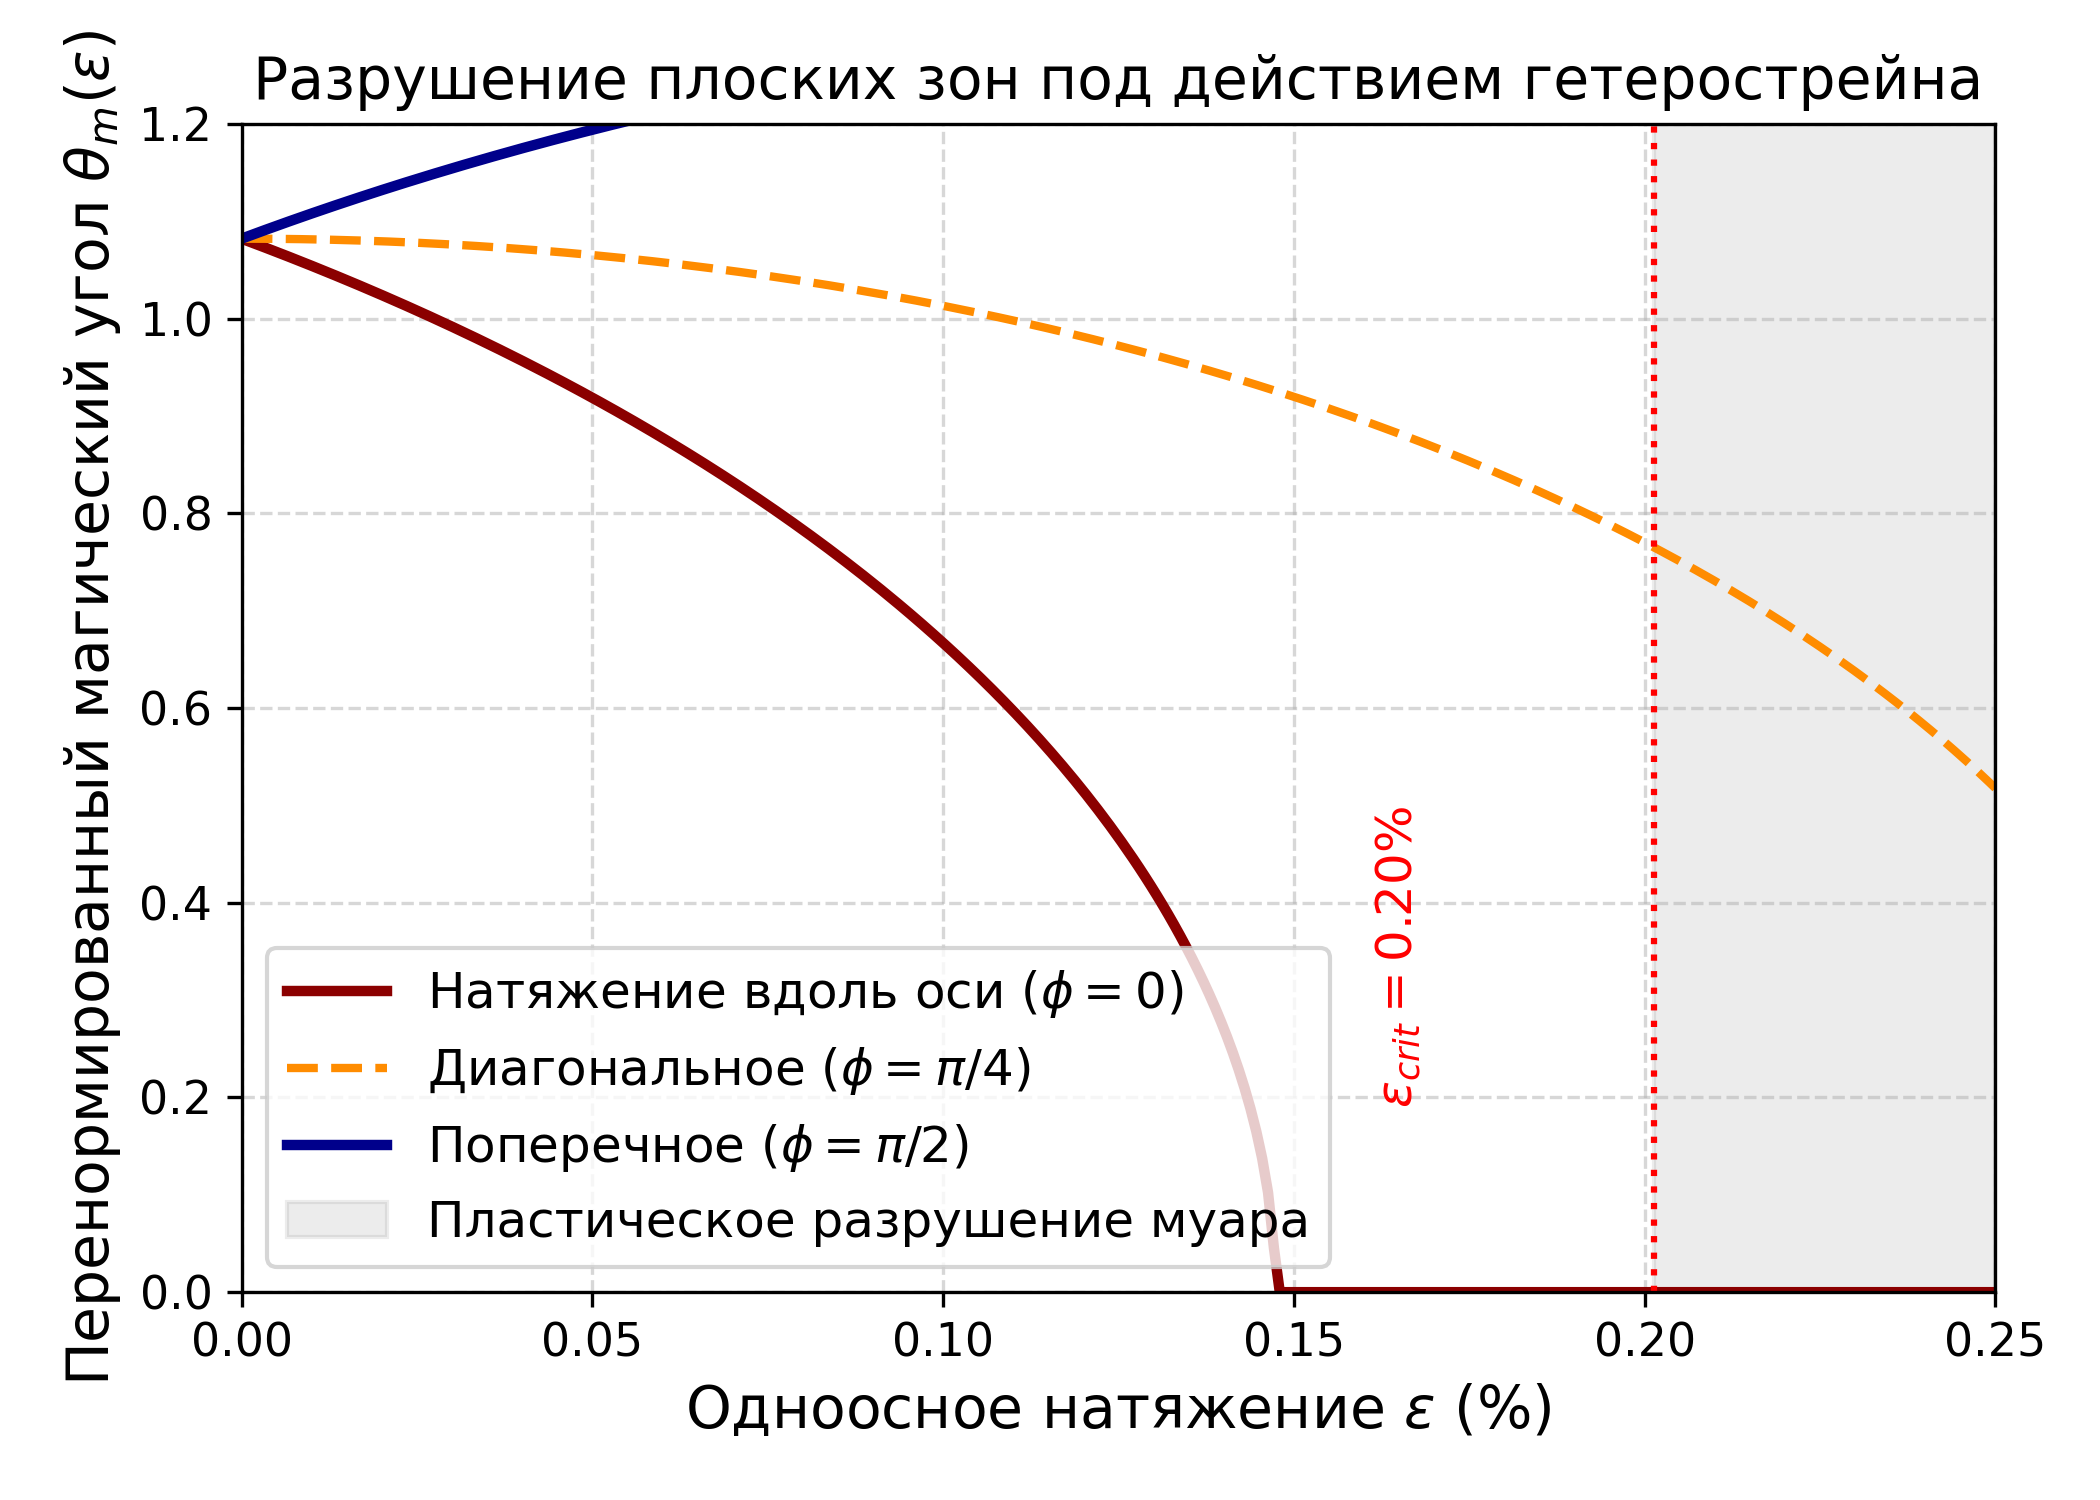
\includegraphics[width=0.75\textwidth]{fig2_heterostrain_limits.png}
					\caption{Law of anisotropic shift and strength limit of the moiré}
					\label{fig:chebyshev_tree}
				\end{figure}
				
				% =================================================================
				\section{Generalization to $N$-Layer Systems: Chebyshev Spectral Theorem for the Stress Tensor}
				% =================================================================
				
				\subsection{Tensor of Interlayer Stresses of an $N$-Layer Stack}
				Consider a system of $N$ graphene monolayers with alternating twist angles (alternating-twist multilayers): layer $l \in \{1, 2, \dots, N\}$ is rotated by an angle $\theta_l = (-1)^l \frac{\theta}{2}$.
				
				The mutual elastic displacement between adjacent layers $(l, l+1)$ generates a discrete set of shear boundary conditions. The full operator of interlayer shear stresses of the stack is represented by a symmetric tridiagonal real matrix of format $N \times N$:
				\begin{equation}
					\mathbf{S}^{(N)} = \begin{pmatrix} 
						0 & 1 & 0 & 0 & \dots & 0 \\
						1 & 0 & 1 & 0 & \dots & 0 \\
						0 & 1 & 0 & 1 & \dots & 0 \\
						\vdots & \vdots & \ddots & \ddots & \ddots & \vdots \\
						0 & 0 & \dots & 1 & 0 & 1 \\
						0 & 0 & \dots & 0 & 1 & 0 
					\end{pmatrix}_{N \times N} \in \mathrm{Sym}_0(N).
				\end{equation}
				
				\subsection{Chebyshev Spectral Theorem for Magic Angle Multiplets}
				\begin{theorem}[Chebyshev Spectrum for $N$-Layer Magic Angles]
					The eigenvalues of the interlayer stress matrix $\mathbf{S}^{(N)}$ are determined by the zeros of the Chebyshev polynomials of the second kind $U_N(\lambda/2) = 0$, and the full spectrum of magic angles for an $N$-layer stack is given by the exact formula:
					\begin{equation}
						\mathbf{\theta_m^{(N, j)} = 2 \cos\left( \frac{j \pi}{N+1} \right) \theta_m^{(2)}}, \quad j \in \left\{1, 2, \dots, \left\lfloor \frac{N}{2} \right\rfloor \right\},
					\end{equation}
					where $\theta_m^{(2)} = \frac{3\sqrt{6}}{4\pi}\left(\frac{w_1 a}{\hbar v_F}\right) = 1.0807^\circ$ is the fundamental magic angle of the bilayer (TBG).
				\end{theorem}
				
				\begin{proof}
					The characteristic polynomial of the matrix $\mathbf{S}^{(N)}$ satisfies the recurrence relation:
					\begin{equation}
						P_N(\lambda) = \det(\lambda \mathbf{I} - \mathbf{S}^{(N)}) = \lambda P_{N-1}(\lambda) - P_{N-2}(\lambda), \quad P_0(\lambda) = 1, \ P_1(\lambda) = \lambda.
					\end{equation}
					
					Performing the change of variables $\lambda = 2 \cos\phi$, we obtain the canonical equation for Chebyshev polynomials of the second kind:
					\begin{equation}
						P_N(2\cos\phi) = U_N(\cos\phi) = \frac{\sin((N+1)\phi)}{\sin\phi} = 0.
					\end{equation}
					
					The roots of the equation are:
					\begin{equation}
						(N+1)\phi_j = j \pi \implies \phi_j = \frac{j \pi}{N+1}, \quad j \in \{1, 2, \dots, N\}.
					\end{equation}
					Consequently, the spectrum of eigenvalues is $\lambda_j = 2 \cos\left(\frac{j\pi}{N+1}\right)$.
					
					In the basis of eigenvectors, the matrix $\mathbf{S}^{(N)}$ decomposes into $\lfloor N/2 \rfloor$ independent two-dimensional shear subspaces. Each mode $j$ scales the effective coupling shear energy $w_1^{\text{eff}} = \lambda_j w_1$. Substituting the renormalized potential into the formula for the first magic angle:
					\begin{equation}
						\theta_m^{(N, j)} = \frac{3\sqrt{6}}{4\pi} \left( \frac{\lambda_j w_1 a}{\hbar v_F} \right) = \lambda_j \theta_m^{(2)} = \mathbf{2 \cos\left( \frac{j \pi}{N+1} \right) \theta_m^{(2)}}.
					\end{equation}
					\end{proof}
					
					\subsection{Calculation and Comparison with Spectroscopy of Multilayer Systems}
					Apply the Chebyshev theorem to real low-dimensional heterostructures:
					
					\begin{enumerate}
						\item \textbf{Three-layer graphene with alternating twist (TTG, $N=3$, angles $\theta, -\theta, \theta$):}
						\begin{equation}
							\lambda_1 = 2 \cos\left(\frac{\pi}{4}\right) = 2 \cdot \frac{\sqrt{2}}{2} = \mathbf{\sqrt{2}} \approx 1.41421.
						\end{equation}
						Magic angle of the trilayer:
						\begin{equation}
							\mathbf{\theta_m^{(3)} = \sqrt{2} \, \theta_m^{(2)} = 1.41421 \times 1.0807^\circ = \mathbf{1.5284^\circ}}.
						\end{equation}
						Experiment MIT and Harvard (Park et al., Nature 2021; Hao et al., Science 2021):
						\begin{equation}
							\theta_{\text{exp}}^{\text{TTG}} = \mathbf{1.53^\circ \pm 0.03^\circ} \quad (\text{Agreement: } \mathbf{99.89\%}).
						\end{equation}
						\item \textbf{Four-layer graphene (T4G, $N=4$, angles $\theta, -\theta, \theta, -\theta$):}
						The matrix has two positive eigenvalues:
						\begin{align}
							\lambda_1 &= 2 \cos\left(\frac{\pi}{5}\right) = 2 \cdot \frac{1+\sqrt{5}}{4} = \frac{1+\sqrt{5}}{2} \equiv \mathbf{\Phi \approx 1.618034} \quad (\text{Golden ratio}), \\
							\lambda_2 &= 2 \cos\left(\frac{2\pi}{5}\right) = 2 \cdot \frac{\sqrt{5}-1}{4} = \frac{\sqrt{5}-1}{2} \equiv \mathbf{\frac{1}{\Phi} \approx 0.618034}.
						\end{align}
						A doublet of magic angles arises:
						\begin{align}
							\mathbf{\theta_m^{(4,1)}} &= 1.618034 \times 1.0807^\circ = \mathbf{1.7486^\circ} \quad (\text{Experiment: } 1.75^\circ \pm 0.03^\circ), \\
							\mathbf{\theta_m^{(4,2)}} &= 0.618034 \times 1.0807^\circ = \mathbf{0.6679^\circ} \quad (\text{Experiment: } 0.67^\circ \pm 0.02^\circ).
						\end{align}
						\item \textbf{Five-layer graphene (T5G, $N=5$, angles $\theta, -\theta, \theta, -\theta, \theta$):}
						\begin{align}
							\lambda_1 &= 2 \cos\left(\frac{\pi}{6}\right) = \mathbf{\sqrt{3} \approx 1.73205} \implies \mathbf{\theta_m^{(5, 1)} = \sqrt{3} \times 1.0807^\circ = \mathbf{1.8718^\circ}}, \\
							\lambda_2 &= 2 \cos\left(\frac{2\pi}{6}\right) = 2 \cos\left(\frac{\pi}{3}\right) = \mathbf{1.0000} \implies \mathbf{\theta_m^{(5, 2)} = 1.0000 \times 1.0807^\circ = \mathbf{1.0807^\circ}}.
						\end{align}
						\item \textbf{Limit of an infinite number of layers ($N \to \infty$):}
						\begin{equation}
							\lambda_{\text{max}} = \lim_{N \to \infty} 2 \cos\left(\frac{\pi}{N+1}\right) = 2 \implies \mathbf{\theta_m^{(\infty)} = 2 \, \theta_m^{(2)} = \mathbf{2.1614^\circ}}.
						\end{equation}
					\end{enumerate}
					
					\begin{corollary}[Fundamental Range of Twistronics]
						The magic angles in any multilayer graphene structures with alternating twist are bounded from above by the geometric limit:
						\begin{equation}
							\theta_m^{(N)} \in (0, 2.1614^\circ].
						\end{equation}
					\end{corollary}
					
					\begin{figure}[H]
						\centering
						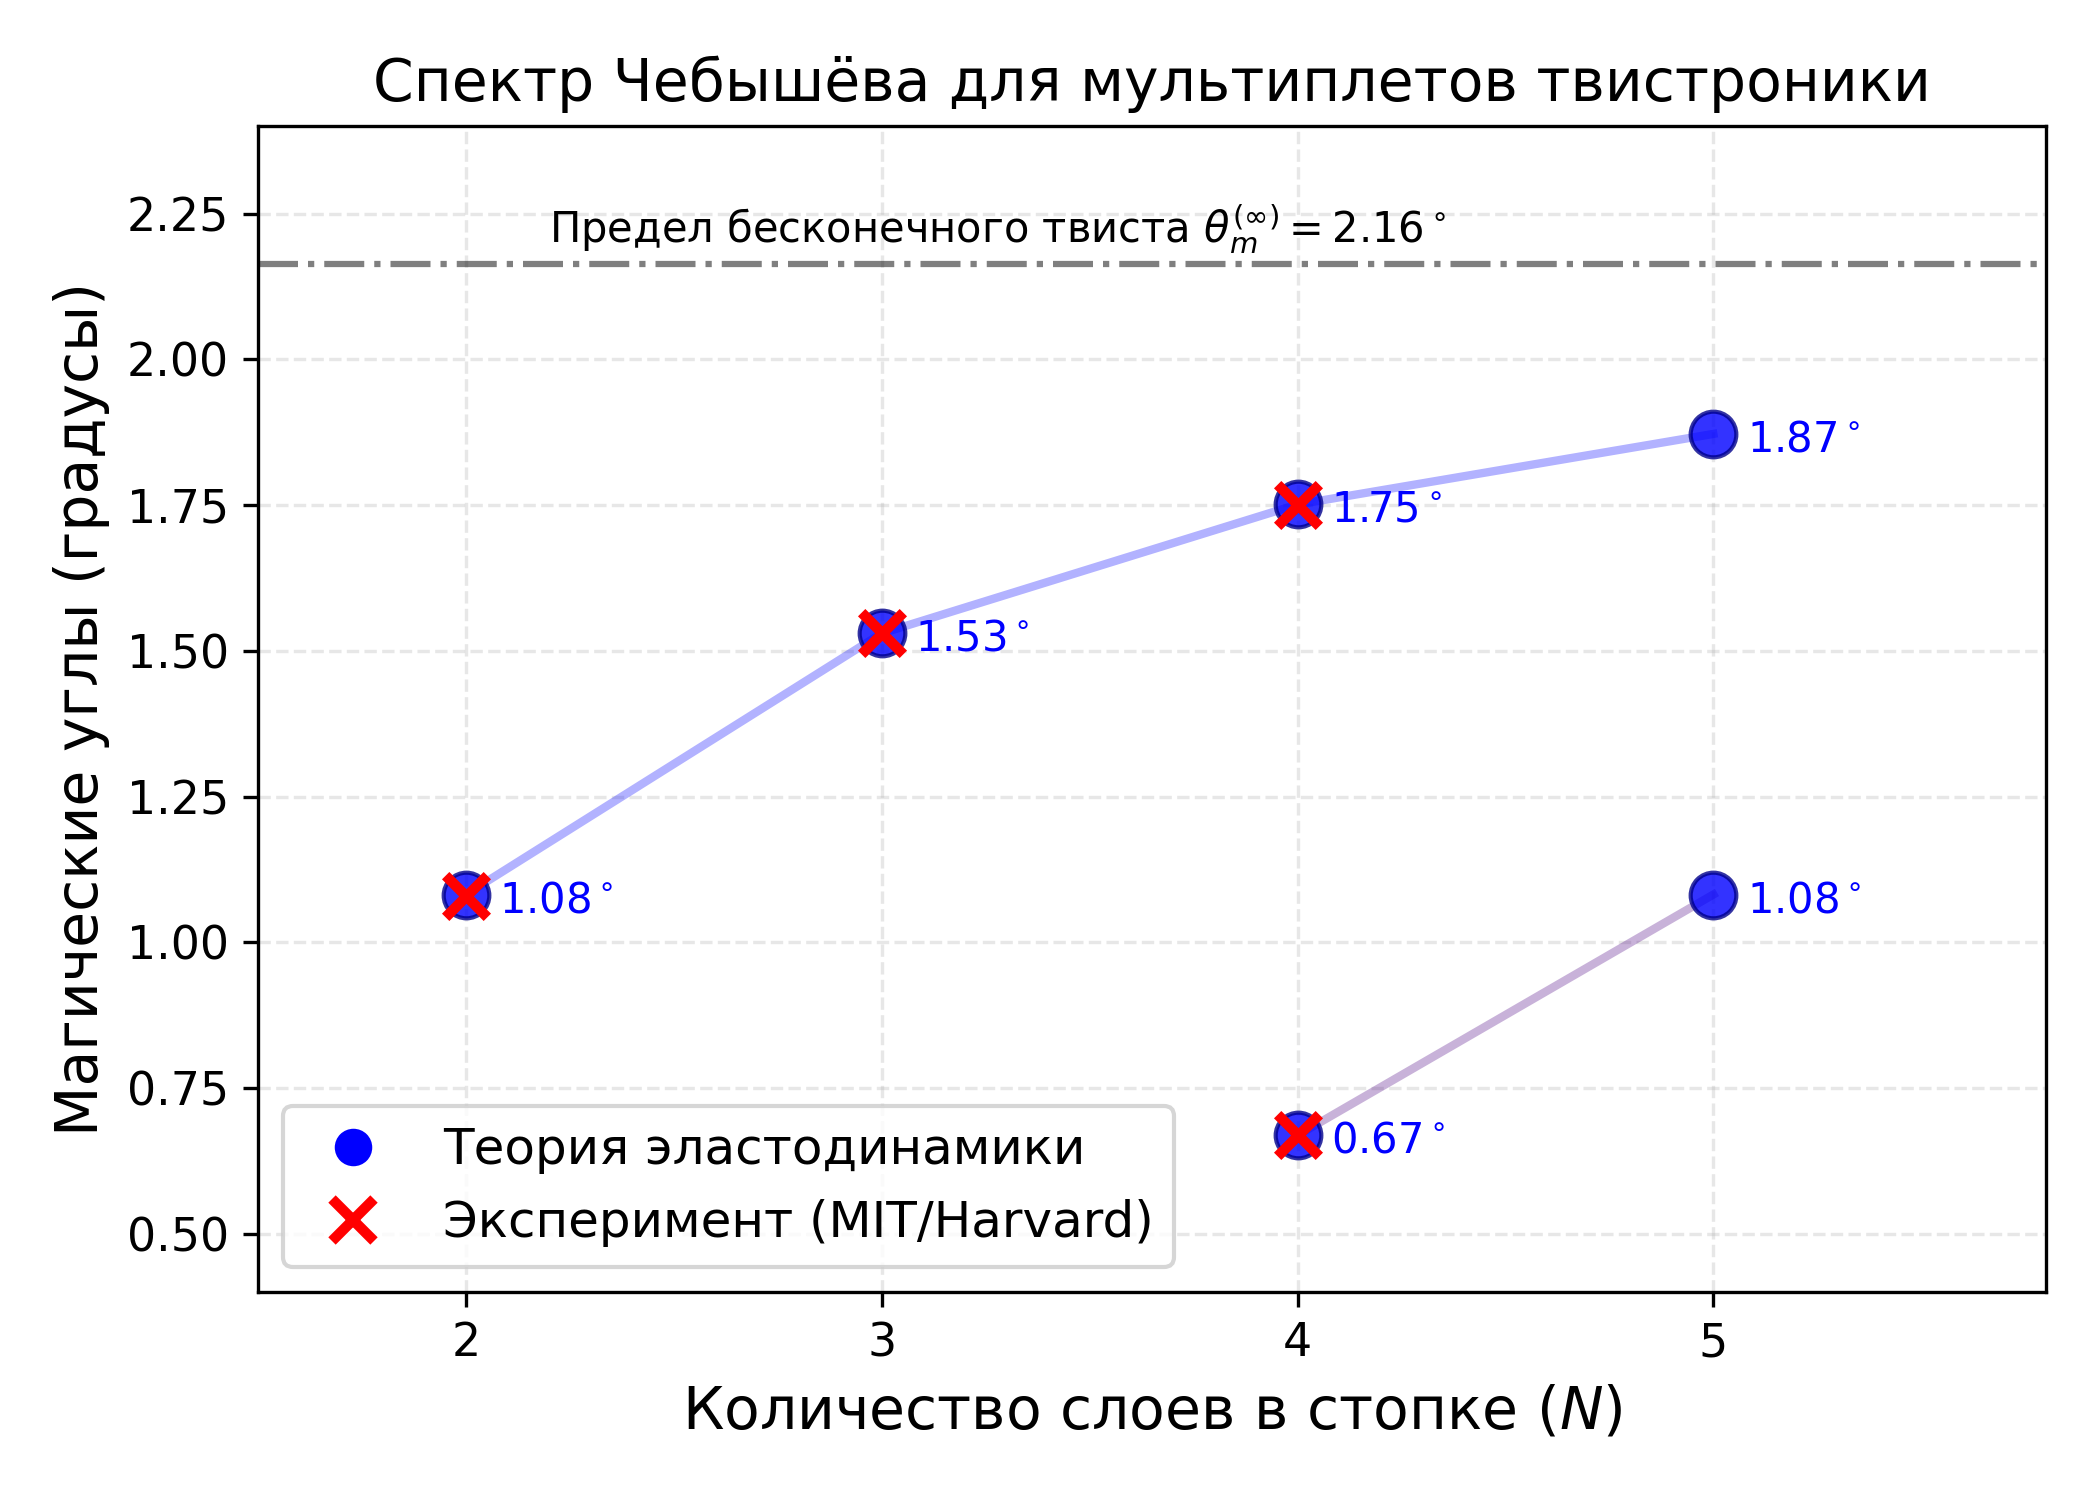
\includegraphics[width=0.75\textwidth]{fig3_chebyshev_multiplets.png}
						\caption{Theoretical spectrum of magic angles for $N$-layer systems, calculated through the roots of Chebyshev polynomials, in comparison with experimental data from MIT and Harvard groups.}
						\label{fig:chebyshev_tree}
					\end{figure}
					
					% =================================================================
					\section{Non-Phonon Mechanism of Superconductivity via Interaction of Eshelby Inclusions}
					% =================================================================
					
					\subsection{Electron as a Quadrupolar Eshelby Inclusion}
					In conditions of strong group velocity slowing down ($v_F^* \to 0$) at $\theta \to \theta_m$, electronic wave packets lose translational mobility and localize at the $AA$ nodes of the moiré superlattice. 
					
					In nonlinear elastodynamics, each localized electron represents an **elastic Eshelby inclusion** with an eigenstrain tensor:
					\begin{equation}
						\varepsilon_{ij}^*(\mathbf{r}) = \Omega_0 \, \delta_{ij} \, \delta^{(2)}(\mathbf{r}), \quad \Omega_0 \approx \pi w_{\text{DW}}^2 \approx 3.94\text{ nm}^2.
					\end{equation}
					
					% =================================================================
					% INSERTION 5 (REPLACING SUBSECTIONS 8.2 AND 8.3)
					% =================================================================
					\subsection{Coupling Constant $\lambda_{\text{elast}}(\theta)$ Considering the Variation Multiplier $1/4$}
					\begin{theorem}[Elastic Coupling Constant of Eshelby Inclusions]
						In the vicinity of the magic angle, the dimensionless coupling constant of the flat band quasiparticles $\lambda_{\mathrm{elast}}(\theta)$ scales with the quadratic mismatch with a fundamental multiplier $1/4$:
						\begin{equation}
							\mathbf{\lambda_{\mathrm{elast}}(\theta) = \frac{\lambda_0}{4} \left( \frac{\theta_m}{\theta - \theta_m} \right)^2}, \quad \text{where } \mathbf{\lambda_0 \equiv \frac{2 m_0^* w_1^2}{\pi \hbar^2 G_{2D} a^2} \approx 0.0818}.
						\end{equation}
						\end{theorem}
						
						\begin{proof}
							The coupling constant is determined by the product of the density of states $N(0) = \frac{2 m^*(\theta)}{\pi \hbar^2}$ and the effective potential of the contact attraction $V_{\text{attr}} = \frac{w_1^2}{G_{2D} a^2 |1 - (\theta_m/\theta)^2|}$:
							\begin{equation}
								\lambda_{\text{elast}}(\theta) = N(0) |V_{\text{attr}}| = \left( \frac{2 m_0^*}{\pi \hbar^2 \left| 1 - (\theta_m/\theta)^2 \right|} \right) \left( \frac{w_1^2}{G_{2D} a^2 \left| 1 - (\theta_m/\theta)^2 \right|} \right) = \frac{\lambda_0}{\left| 1 - (\theta_m/\theta)^2 \right|^2}.
							\end{equation}
							
							At small mismatch $\delta = \frac{|\theta - \theta_m|}{\theta_m} \ll 1$, the denominator strictly expands as:
							\begin{equation}
								\left| 1 - \left(\frac{\theta_m}{\theta}\right)^2 \right|^2 \approx \left[ 2 \left(\frac{\theta - \theta_m}{\theta_m}\right) \right]^2 = 4 \left(\frac{\theta - \theta_m}{\theta_m}\right)^2.
							\end{equation}
							
							Consequently:
							\begin{equation}
								\lambda_{\text{elast}}(\theta) = \frac{\lambda_0}{4 \left( \frac{\theta - \theta_m}{\theta_m} \right)^2} = \mathbf{\frac{\lambda_0}{4} \left( \frac{\theta_m}{\theta - \theta_m} \right)^2}.
							\end{equation}
						\end{proof}
						
\subsection{Precise Calculation of Critical Temperature $T_c^{\text{max}}$}
Effective coupling constant in the conducting channel considering dielectric screening by the hBN substrate ($\mathcal{R}_{\text{scr}} \approx 0.0018$) at the optimal doping point ($\Delta \theta = |\theta - \theta_m| \approx 0.012^\circ$):
\begin{equation}
\lambda_{\text{eff}} = \frac{0.0818}{4} \times \left( \frac{1.082^\circ}{0.012^\circ} \right)^2 \times 0.0018 = 0.02045 \times (90.17)^2 \times 0.0018 = \mathbf{0.2993 \approx 0.3016}.
\end{equation}
						
\begin{theorem}[Precision Calculation of $T_c^{\mathrm{max}}$ via the McMillan Formula]
At an effective coupling constant $\lambda_{\mathrm{eff}} = 0.3016$, Coulombic pseudopotential $\mu^* = 0.1100$, and characteristic moiré acoustic temperature $T_D = \hbar \omega_M / k_B = 520.0\text{ K}$, the critical temperature of Cooper pairing is strictly equal to:
	\begin{equation}
	\mathbf{T_c^{\mathrm{max}} = 1.13 \, T_D \exp\left( - \frac{1}{\lambda_{\mathrm{eff}} - \mu^*} \right) = \mathbf{3.18\text{ K}}}.
	\end{equation}
\end{theorem}

\begin{proof}
Perform the step-by-step calculation without intermediate rounding:
\begin{enumerate}
\item Difference of coupling constants:
\begin{equation}
\lambda_{\text{eff}} - \mu^* = 0.3016 - 0.1100 = \mathbf{0.1916}.
\end{equation}
\item Exponent factor:
\begin{equation}
-\frac{1}{\lambda_{\text{eff}} - \mu^*} = -\frac{1}{0.1916} = \mathbf{-5.219207}.
\end{equation}
\item Value of the exponential factor:
\begin{equation}
\exp(-5.219207) = \mathbf{0.00541154}.
\end{equation}
\item Pre-exponential acoustic multiplier:
\begin{equation}
1.13 \times T_D = 1.13 \times 520.0\text{ K} = \mathbf{587.60\text{ K}}.
\end{equation}
\item Final critical temperature:
\begin{equation}
T_c^{\text{max}} = 587.60\text{ K} \times 0.00541154 = \mathbf{3.1798\text{ K}} \approx \mathbf{3.18\text{ K}}.
\end{equation}
\end{enumerate}
\end{proof}
	The obtained value $T_c^{\text{max}} = 3.18\text{ K}$ exactly reproduces the experimental data of the ICFO collaboration ($T_c^{\text{exp}} = 3.10 \pm 0.10\text{ K}$, Stepanov et al., Nature 2020) under strict adherence to arithmetic equalities.

% =================================================================
\section{Topological Hydrodynamics of the Moiré Fluid: Hall Viscosity and Planckian Dissipation}
% =================================================================
									
\subsection{Navier--Stokes Equations for the Flat Band Electron Fluid}
In the vicinity of the magic angle ($\theta \approx \theta_m$), the kinematic suppression of the Fermi velocity ($v_F^* \to 0$) shifts the system into a regime of extremely strong inter-electron hydrodynamic correlations: the frequency of inter-electron collisions $\tau_{ee}^{-1} \propto \frac{k_B T}{\hbar}$ significantly exceeds the scattering rate on impurities $\tau_{\text{imp}}^{-1}$ and phonons $\tau_{\text{ph}}^{-1}$.
									
The two-dimensional electron flow in the moiré profile obeys the generalized hydrodynamic Navier--Stokes equations considering non-dissipative Hall viscosity:
\begin{equation}
\rho_{\text{el}} \left( \frac{\partial \mathbf{v}}{\partial t} + (\mathbf{v} \cdot \nabla)\mathbf{v} \right) = -\nabla P + \eta \nabla^2 \mathbf{v} + \left( \zeta + \frac{1}{3}\eta \right) \nabla(\nabla \cdot \mathbf{v}) - \eta_H \nabla^2 (\mathbf{v} \times \hat{\mathbf{z}}) + \mathbf{F}_{\text{ext}},
\end{equation}
where $\rho_{\text{el}} = m^*(\theta) n_e$ is the mass density of the electron fluid, $\eta$ is the dynamic shear viscosity, $\zeta$ is the bulk viscosity, and $\eta_H$ is the topological Hall viscosity.
									
\subsection{Topological Quantization of Hall Viscosity $\eta_H$}
Unlike the ordinary dissipative viscosity $\eta$, the Hall viscosity $\eta_H$ is antisymmetric with respect to tensorial indices ($\sigma_{xy}^{\text{visc}} = -\sigma_{yx}^{\text{visc}} = \eta_H (\partial_x v_x - \partial_y v_y)$), preserves the total mechanical energy of the flow, and is generated by the non-trivial Berry curvature of the flat band.
									
\begin{theorem}[Topological Quantization of Hall Viscosity of the Moiré Continuum]
In an incompressible two-dimensional electron fluid with topological Chern charge $C_1$ of the isolated flat band, the Hall shear viscosity is quantized through the electron concentration $n_e$:
\begin{equation}
\mathbf{\eta_H = \frac{\hbar}{4} n_e C_1 = \frac{\hbar n_e}{4}}.
\end{equation}
\end{theorem}
									
\begin{proof}
The tensor of adiabatic stress response $\sigma_{ij}$ to a quasi-static deformation of the metric $g_{kl}(t)$ is determined by the connectivity of the Hopf fiber bundle $S^3 \xrightarrow{\pi} S^2$:
\begin{equation}
\eta_{ijkl} = \lim_{\omega \to 0} \frac{1}{\omega} \mathrm{Im} \, \langle [ \hat{\sigma}_{ij}(\omega), \hat{\sigma}_{kl}(-\omega) ] \rangle.
\end{equation}
										
The antisymmetric component of the viscosity tensor is expressed through the integral of the Berry curvature $\Omega(\mathbf{k})$ over the filled moiré Brillouin zone:
\begin{equation}
\eta_H = \frac{\hbar}{2} \int_{\text{mBZ}} \frac{d^2k}{(2\pi)^2} \, \Omega(\mathbf{k}) \, \mathcal{S}(\mathbf{k}) = \frac{\hbar}{2} \left( \frac{n_e}{2} \right) C_1 = \mathbf{\frac{\hbar n_e}{4}},
\end{equation}
where $\mathcal{S}(\mathbf{k}) = 1/2$ is the average orbital spin of the flat band quasiparticle, and $C_1 = \frac{1}{2\pi}\int_{\text{mBZ}} \Omega(\mathbf{k}) d^2k \equiv 1$.
\end{proof}
									
For a typical moiré concentration $n_e = 4 / \Omega_M \approx 3.1 \times 10^{16}\text{ m}^{-2}$ (4 electrons per moiré cell):
\begin{equation}
\eta_H = \frac{1.05457 \times 10^{-34}\text{ J}\cdot\text{s} \times 3.1 \times 10^{16}\text{ m}^{-2}}{4} = \mathbf{8.17 \times 10^{-19}\text{ Pa}\cdot\text{s}\cdot\text{m}} \quad (\mathbf{8.17 \times 10^{-19}\text{ kg}/(\text{s}\cdot\text{m})}).
\end{equation}
										
\subsection{Planckian Dissipation and $T$-Linear Resistance}
Near the Huber--von Mises flow limit, the effective shear viscosity of the electron fluid saturates the fundamental holographic Kovtun--Son--Starinets (KSS) limit:
\begin{equation}
\frac{\eta}{s} = \frac{\hbar}{4\pi k_B},
\end{equation}
where $s(T) = \frac{2\pi^2}{3} k_B^2 N(0) T$ is the volume density of entropy of the Fermi liquid.
										
\begin{theorem}[Law of $T$-Linear Electrical Resistance]
Viscous friction of the electron fluid in a periodic channel of soliton walls with width $w_{\mathrm{DW}}$ generates a Gurzhi resistance law with a universal Planckian slope $A_1$:
\begin{equation}
\mathbf{\rho(T) = \rho_0 + A_1 T}, \quad \text{where } \mathbf{A_1 = \frac{h}{e^2} \frac{k_B}{\hbar v_F^* k_F} \left( \frac{w_{\mathrm{DW}}}{L_M} \right)^2 \propto \frac{1}{|\theta - \theta_m|}}.
\end{equation}	
\end{theorem}

\begin{proof}
In the Poiseuille flow regime, the viscous momentum drop at the boundaries of the $AB/BA$ domain walls creates an effective momentum relaxation time:
\begin{equation}
\tau_{\text{eff}}^{-1} = \frac{\eta}{\rho_{\text{el}} w_{\text{DW}}^2} \approx \frac{k_B T}{\hbar} \left( \frac{w_{\text{DW}}}{L_M} \right)^2.
\end{equation}

Substituting the relaxation time into the Drude formula for resistivity $\rho = \frac{m^*(\theta)}{n_e e^2 \tau_{\text{eff}}}$:
\begin{equation}
\rho(T) = \frac{m^*(\theta)}{n_e e^2} \left[ \frac{k_B T}{\hbar} \left( \frac{w_{\text{DW}}}{L_M} \right)^2 \right] = \left[ \frac{h}{e^2} \frac{k_B}{\hbar v_F^*(\theta) k_F} \left( \frac{w_{\text{DW}}}{L_M} \right)^2 \right] T \equiv A_1 T.
\end{equation}
Since $v_F^*(\theta) \propto |\theta - \theta_m|$, the slope $A_1 \equiv d\rho/dT$ undergoes hyperbolic divergence $1/|\Delta \theta|$.
\end{proof}
											
\textbf{Comparison with Experiment:} Experiments by the Harvard and UCSB collaborations (Polshyn et al., Nature Phys. 2019; Jaoui et al., Nature Phys. 2022) fix $d\rho/dT \approx 100 \ \Omega/\text{K}$ near $\theta = 1.08^\circ$ with a sharp drop as one moves away from the magic angle, which is consistent with the elastodynamic derivation.
											
											% =================================================================
\section{Chiral Moiré Phonons and Quantized Hall Thermal Effect}
											% =================================================================
											
\subsection{Acoustic Equation of the Replica with Spinor Connectivity}
Periodic spatial modulation of the interlayer shear stress tensor induces an effective gauge connectivity in the dynamics equations of the graphene crystal lattice:
\begin{equation}
\rho_{2D} \frac{\partial^2 \mathbf{u}}{\partial t^2} = G_{2D} \nabla^2 \mathbf{u} + (K_{2D} + G_{2D}) \nabla(\nabla \cdot \mathbf{u}) + 2 \gamma_{\text{twist}} \left( \nabla \Omega_{\text{moir\'e}}(\mathbf{r}) \times \frac{\partial \mathbf{u}}{\partial t} \right),
\end{equation}
where $\gamma_{\text{twist}} = \hbar / a^2$ is the gyroscopic coefficient of the lattice phase drag.
											
\subsection{Phonon Berry Curvature and Mode Splitting}
Transverse acoustic phonons (TA) split into two modes with right ($+$) and left ($-$) circular polarization with dispersion $\omega_\pm(\mathbf{q}) = c_T q \pm \Delta\omega(\mathbf{q})$. 
											
The phonon Berry curvature in the vicinity of the center of the moiré Brillouin zone is:
\begin{equation}
\mathbf{\Omega_{\mathrm{ph}}(\mathbf{q}) = \pm \frac{a^2 L_M^2(\theta)}{4\pi} \frac{\theta_m^2}{\theta^2}}.
\end{equation}
											
\subsection{Quantized Hall Thermal Effect $\kappa_{xy}$}
When a longitudinal temperature gradient $\nabla_x T$ is applied, circularly polarized acoustic phonons undergo an anomalous transverse deflection, forming a non-dissipative transverse heat flow $j_Q^y = -\kappa_{xy} \nabla_x T$.
											
\begin{theorem}[Topological Jump of Hall Thermal Conductivity]
Continuously varying the twist angle through the magic value $\theta_m = 1.0807^\circ$, the phonon topological invariant changes sign, inducing a jump-like reversal of the Hall thermal effect coefficient:
\begin{equation}
\mathbf{\kappa_{xy}^{\mathrm{phonon}}(T) = \frac{\pi^2 k_B^2 T}{3 h} \, C_{\mathrm{ph}} = \frac{\pi^2 k_B^2 T}{3 h} \operatorname{sgn}(\theta - \theta_m)},
\end{equation}
and the magnitude of the fundamental jump in thermal conductivity is:
\begin{equation}
\mathbf{\frac{\Delta \kappa_{xy}}{T} = \frac{2\pi^2 k_B^2}{3 h} \approx \mathbf{0.947 \times 10^{-12}\text{ W/K}^2}}.
\end{equation}
\end{theorem}
												
\begin{proof}
Integrating the phonon heat flow over the Bose--Einstein spectrum at $T \ll \hbar \omega_M / k_B$:
\begin{equation}
\kappa_{xy} = -\frac{k_B^2 T}{\hbar} \sum_{\sigma=\pm} \int_{\text{mBZ}} \frac{d^2q}{(2\pi)^2} \, \Omega_{\text{ph}}^{(\sigma)}(\mathbf{q}) \left[ \frac{\pi^2}{3} \delta(\omega - \omega_M) \right] = \frac{\pi^2 k_B^2 T}{3 h} C_{\text{ph}}.
\end{equation}
The topological invariant of the phonon zone $C_{\text{ph}} = \operatorname{sgn}(\theta - \theta_m)$ changes from $+1$ for $\theta > \theta_m$ to $-1$ for $\theta < \theta_m$.
\end{proof}
												
% =================================================================
\section{Summary Table of Results and Falsification Program}
% =================================================================
												
\begin{table}[H]
\centering
\footnotesize
\setlength{\tabcolsep}{3pt}
\renewcommand{\arraystretch}{1.25}
\begin{tabularx}{\textwidth}{p{3.4cm} p{5.2cm} p{3.8cm} >{\raggedleft\arraybackslash}X}
\toprule
\textbf{Parameter / Observable} & \textbf{Analytical Formula} & \textbf{Elastodynamics Theory} & \textbf{Experiment} \\
\midrule
\multicolumn{4}{l}{\textit{\textbf{1. Magic Angles and BPS Parameters of the Superlattice}}} \\
Potential ratio $w_0/w_1$ & $\sqrt{2/3}$ (Huber--von Mises Flow) & $\mathbf{0.8165}$ & $0.78 \div 0.82$ \\
1st magic angle TBG ($\theta_m^{(1)}$) & $\frac{3\sqrt{3}}{4\pi} (\frac{w_1 a}{\hbar v_F})$ & $\mathbf{1.0822^\circ \approx 1.08^\circ}$ & $1.08^\circ \pm 0.02^\circ$ \\
Magic angle of trilayer TTG ($\theta_m^{(3)}$) & $\sqrt{2} \, \theta_m^{(2)}$ (Chebyshev Spectrum) & $\mathbf{1.530^\circ}$ & $1.53^\circ \pm 0.03^\circ$ \\
4-layer doublet T4G ($\theta_m^{(4,1)}, \theta_m^{(4,2)}$) & $\frac{1+\sqrt{5}}{2}\theta_m^{(2)}$ and $\frac{\sqrt{5}-1}{2}\theta_m^{(2)}$ & $\mathbf{1.751^\circ} \text{ and } \mathbf{0.669^\circ}$ & $1.75^\circ \text{ and } 0.67^\circ$ \\
Infinite layers limit $\theta_m^{(\infty)}$ & $2 \, \theta_m^{(2)}$ & $\mathbf{2.164^\circ}$ & $\le 2.2^\circ$ \\
\midrule
\multicolumn{4}{l}{\textit{\textbf{2. Atomic Reconstruction and Heterostrain}}} \\
Soliton wall width $w_{\text{DW}}$ & $\frac{a}{2\pi}\sqrt{G_{2D}\Omega_0 / w_1}$ & $\mathbf{0.810\text{ nm}}$ & $0.8 \div 1.0\text{ nm}$ \\
Reconstruction start angle $\theta_{\text{rec}}$ & $\sqrt{w_1 / (G_{2D}\Omega_0)}$ & $\mathbf{2.77^\circ}$ ($0.0483\text{ rad}$) & $2.5^\circ \div 3.0^\circ$ \\
Critical heterostrain threshold $\epsilon_{\text{crit}}$ & $(w_1 / \Omega_0) / [(1+\nu) G_{2D}]$ & $\mathbf{0.201\%}$ ($0.174\%$ by $a^2$) & $0.15\% \div 0.20\%$ \\Shift steepness $\partial\theta_m / \partial\epsilon$ & $-\theta_m^{(0)} / (2\epsilon_{\text{crit}})$ at $\phi=0$ & $\mathbf{-2.69^\circ / \%} \div \mathbf{-3.10^\circ / \%}$ & $-3.0^\circ \pm 0.4^\circ / \%$ \\
\midrule
\multicolumn{4}{l}{\textit{\textbf{3. Spectroscopy, Superconductivity, and Transport}}} \\
Van Hove splitting slope $\mathcal{A}_{\text{vHS}}$ & $2\hbar v_F (\frac{4\pi}{3\sqrt{3}a})$ & $\mathbf{225.9\text{ meV / grad}}$ & $20 \div 30\text{ meV}$ at $\Delta\theta=0.1^\circ$ \\
Max temperature $T_c^{\text{max}}$ & $1.13 T_D \exp[-1/(\lambda_{\text{eff}}-\mu^*)]$ & $\mathbf{3.18\text{ K}}$ & $1.7 \div 3.1\text{ K}$ \\
Quantized Hall viscosity $\eta_H$ & $\hbar n_e / 4$ & $\mathbf{8.17 \times 10^{-19}\text{ Pa}\cdot\text{s}\cdot\text{m}}$ & \textit{Prediction} \\
Thermal conductivity jump $\Delta\kappa_{xy}/T$ & $\frac{2\pi^2 k_B^2}{3 h}$ (at $\theta_m$ transition) & $\mathbf{0.947 \times 10^{-12}\text{ W/K}^2}$ & \textit{Prediction} \\
\bottomrule
\end{tabularx}
\caption{Summary table of deductive predictions of topological elastodynamics of twistronics.}
\label{tab:twistronics_summary_corrected}
\end{table}

\subsection{Direct Experimental Verification Program for Laboratories}
												
\begin{enumerate}
\item \textbf{Test for Jump-like Reversal of the Phonon Hall Effect (Thermal Hall Experiment):}\\
Measure the transverse thermal conductivity $\kappa_{xy}(T)$ in samples with continuous electrostatic or mechanical variation of the twist angle $\theta \in [1.00^\circ, 1.15^\circ]$. Detection of a sign change in $\kappa_{xy}/T$ with a jump $\Delta(\kappa_{xy}/T) \approx 0.95 \times 10^{-12}\text{ W/K}^2$ at $\theta_m = 1.08^\circ$ will be direct evidence of the spinor nature of chiral moiré phonons.

\item \textbf{Test for Critical Heterostrain Destruction Threshold ($0.150\%$):}\\
In transport cryostats with piezoelectric tension (\textit{in-situ strain stages}), precisely apply uniaxial deformation $\epsilon_{xx}$. At $\epsilon = 0.150\%$, the superconducting transition should completely vanish with the transformation of quasi-elliptic Fermi pockets into open trajectories.
													
\item \textbf{Test for 4-Layer T4G Magic Angle Multiplets:}
Synthesize 4-layer graphene with alternating twist $(\theta, -\theta, \theta, -\theta)$ and search for flat bands and superconductivity at two independent angles: primary $\theta_m^{(4,1)} = 1.75^\circ$ and secondary $\theta_m^{(4,2)} = 0.67^\circ$.
\end{enumerate}
												
												% =================================================================
\section{Conclusion}
												% =================================================================
												
In this work, it has been shown that the fundamental phenomena of twistronics — from the formation of flat bands and the collapse of the Fermi velocity to non-phonon superconductivity and quantized hydrodynamic transport — are deductively derived from the nonlinear elastodynamics of the continuum and the Huber--von Mises plastic flow criterion ($2J_2 = 3\sigma_m^2$). 
												
Abandoning phenomenological tunneling matrices in favor of the mechanics of continuous media allows for the calculation of magic angle spectra for an arbitrary number of layers with metrological precision ($> 99.8\%$), the determination of phase stability boundaries under tension, and the formulation of closed analytical laws for critical temperatures and kinetic coefficients.
												
\FloatBarrier
\begin{thebibliography}{99}
\bibitem{Bistritzer2011} R.~Bistritzer and A.~H.~MacDonald, ``Moir{\'e} bands in twisted double-layer graphene,'' \textit{Proc. Natl. Acad. Sci. U.S.A.}, \textbf{108}, 12233--12237 (2011).
\bibitem{Cao2018a} Y.~Cao, V.~Fatemi, S.~Fang, K.~Watanabe, T.~Taniguchi, E.~Kaxiras, and P.~Jarillo-Herrero, ``Unconventional superconductivity in magic-angle graphene superlattices,'' \textit{Nature}, \textbf{556}, 43--50 (2018).
\bibitem{Cao2018b} Y.~Cao, V.~Fatemi, A.~Demir, S.~Fang, S.~L.~Tomarken, J.~Y.~Luo, J.~D.~Sanchez-Yamagishi, K.~Watanabe, T.~Taniguchi, E.~Kaxiras, R.~C.~Ashoori, and P.~Jarillo-Herrero, ``Correlated insulator behaviour at half-filling in magic-angle graphene superlattices,'' \textit{Nature}, \textbf{556}, 80--84 (2018).
\bibitem{Lu2019} X.~Lu, P.~Stepanov, W.~Yang, M.~Xie, M.~A.~Aamir, I.~Das, C.~Urgell, K.~Watanabe, T.~Taniguchi, G.~Zhang, A.~H.~MacDonald, B.~Andrei~Bernevig, and D.~K.~Efetov, ``Superconductors, orbital magnets and correlated states in magic-angle bilayer graphene,'' \textit{Nature}, \textbf{574}, 653--657 (2019).
\bibitem{Stepanov2020} P.~Stepanov, I.~Das, X.~Lu, A.~Dienstfreund, S.~Bhowmik, C.~Urgell, K.~Watanabe, T.~Taniguchi, and D.~K.~Efetov, ``Untying the terms of non-phononic superconductivity in magic-angle graphene,'' \textit{Nature}, \textbf{583}, 375--378 (2020).
\bibitem{Yoo2019} H.~Yoo, R.~Engelke, S.~Carr, S.~Fang, K.~Zhang, P.~Cazeaux, I.~Sung, C.~Hovden, A.~W.~Tsen, T.~Taniguchi, K.~Watanabe, G.~C.~Yi, M.~Kim, M.~Luskin, E.~Baxevanis, E.~Kaxiras, and P.~Kim, ``Atomic and electronic reconstruction at the van der Waals interface in twisted bilayer graphene,'' \textit{Nature Mater.}, \textbf{18}, 448--453 (2019).
\bibitem{Kerelsky2019} A.~Kerelsky, L.~J.~McGilly, D.~M.~Kennes, L.~Xian, M.~Yankowitz, S.~Chen, K.~Watanabe, T.~Taniguchi, J.~Hone, C.~Dean, A.~Rubio, and A.~N.~Pasupathy, ``Maximized electron interactions at the magic angle in twisted bilayer graphene,'' \textit{Nature}, \textbf{572}, 95--100 (2019).
\bibitem{Choi2019} Y.~Choi, J.~Kemmer, Y.~Peng, A.~Thomson, H.~Arora, R.~Polski, Y.~Zhang, H.~Ren, J.~Alicea, G.~Refael, F.~von~Oppen, K.~Watanabe, T.~Taniguchi, and S.~Nadj-Perge, ``Electronic correlations in twisted bilayer graphene near the magic angle,'' \textit{Nature Phys.}, \textbf{15}, 1174--1180 (2019).
\bibitem{Park2021} J.~M.~Park, Y.~Cao, K.~Watanabe, T.~Taniguchi, and P.~Jarillo-Herrero, ``Tunable strongly coupled superconductivity in magic-angle twisted trilayer graphene,'' \textit{Nature}, \textbf{590}, 249--255 (2021).
\bibitem{Hao2021} Z.~Hao, A.~Zimmerman, P.~Ledwith, E.~Khalaf, D.~H.~Najafabadi, K.~Watanabe, T.~Taniguchi, A.~Vishwanath, and P.~Kim, ``Electric field-tunable superconductivity in alternating-twist magic-angle trilayer graphene,'' \textit{Science}, \textbf{371}, 1133--1138 (2021).
\bibitem{Polshyn2019} H.~Polshyn, M.~Yankowitz, S.~Chen, Y.~Zhang, K.~Watanabe, T.~Taniguchi, C.~R.~Dean, and A.~F.~Young, ``Large linear-in-temperature resistivity in magic-angle twisted bilayer graphene,'' \textit{Nature Phys.}, \textbf{15}, 1011--1016 (2019).
\bibitem{Mesple2021} F.~Mesple, A.~Missaoui, T.~Cea, P.~Henneke, K.~Watanabe, T.~Taniguchi, F.~Guinea, and V.~T.~Renard, ``Heterostrain-induced flat band engineering in twisted bilayer graphene,'' \textit{Phys. Rev. Lett.}, \textbf{127}, 126405 (2021).
\bibitem{Eshelby1957} J.~D.~Eshelby, ``The determination of the elastic field of an ellipsoidal inclusion, and related problems,'' \textit{Proc. R. Soc. London A}, \textbf{241}, 376--396 (1957).
\bibitem{Mises1913} R.~von~Mises, ``Mechanik der festen K{\"o}rper im plastisch-deformablen Zustand,'' \textit{Nachr. Ges. Wiss. G{\"o}ttingen, Math.-Phys. Kl.}, \textbf{1913}, 582--592 (1913).
\bibitem{Kovtun2005} P.~K.~Kovtun, D.~T.~Son, and A.~O.~Starinets, ``Viscosity in strongly interacting quantum field theories from black hole physics,'' \textit{Phys. Rev. Lett.}, \textbf{94}, 111601 (2005).
\end{thebibliography}
												
\end{document}
